\documentclass[twoside]{book}

% Packages required by doxygen
\usepackage{fixltx2e}
\usepackage{calc}
\usepackage{doxygen}
\usepackage[export]{adjustbox} % also loads graphicx
\usepackage{graphicx}
\usepackage[utf8]{inputenc}
\usepackage{makeidx}
\usepackage{multicol}
\usepackage{multirow}
\PassOptionsToPackage{warn}{textcomp}
\usepackage{textcomp}
\usepackage[nointegrals]{wasysym}
\usepackage[table]{xcolor}

% Font selection
\usepackage[T1]{fontenc}
\usepackage[scaled=.90]{helvet}
\usepackage{courier}
\usepackage{amssymb}
\usepackage{sectsty}
\renewcommand{\familydefault}{\sfdefault}
\allsectionsfont{%
  \fontseries{bc}\selectfont%
  \color{darkgray}%
}
\renewcommand{\DoxyLabelFont}{%
  \fontseries{bc}\selectfont%
  \color{darkgray}%
}
\newcommand{\+}{\discretionary{\mbox{\scriptsize$\hookleftarrow$}}{}{}}

% Page & text layout
\usepackage{geometry}
\geometry{%
  a4paper,%
  top=2.5cm,%
  bottom=2.5cm,%
  left=2.5cm,%
  right=2.5cm%
}
\tolerance=750
\hfuzz=15pt
\hbadness=750
\setlength{\emergencystretch}{15pt}
\setlength{\parindent}{0cm}
\setlength{\parskip}{3ex plus 2ex minus 2ex}
\makeatletter
\renewcommand{\paragraph}{%
  \@startsection{paragraph}{4}{0ex}{-1.0ex}{1.0ex}{%
    \normalfont\normalsize\bfseries\SS@parafont%
  }%
}
\renewcommand{\subparagraph}{%
  \@startsection{subparagraph}{5}{0ex}{-1.0ex}{1.0ex}{%
    \normalfont\normalsize\bfseries\SS@subparafont%
  }%
}
\makeatother

% Headers & footers
\usepackage{fancyhdr}
\pagestyle{fancyplain}
\fancyhead[LE]{\fancyplain{}{\bfseries\thepage}}
\fancyhead[CE]{\fancyplain{}{}}
\fancyhead[RE]{\fancyplain{}{\bfseries\leftmark}}
\fancyhead[LO]{\fancyplain{}{\bfseries\rightmark}}
\fancyhead[CO]{\fancyplain{}{}}
\fancyhead[RO]{\fancyplain{}{\bfseries\thepage}}
\fancyfoot[LE]{\fancyplain{}{}}
\fancyfoot[CE]{\fancyplain{}{}}
\fancyfoot[RE]{\fancyplain{}{\bfseries\scriptsize Generated by Doxygen }}
\fancyfoot[LO]{\fancyplain{}{\bfseries\scriptsize Generated by Doxygen }}
\fancyfoot[CO]{\fancyplain{}{}}
\fancyfoot[RO]{\fancyplain{}{}}
\renewcommand{\footrulewidth}{0.4pt}
\renewcommand{\chaptermark}[1]{%
  \markboth{#1}{}%
}
\renewcommand{\sectionmark}[1]{%
  \markright{\thesection\ #1}%
}

% Indices & bibliography
\usepackage{natbib}
\usepackage[titles]{tocloft}
\setcounter{tocdepth}{3}
\setcounter{secnumdepth}{5}
\makeindex

% Hyperlinks (required, but should be loaded last)
\usepackage{ifpdf}
\ifpdf
  \usepackage[pdftex,pagebackref=true]{hyperref}
\else
  \usepackage[ps2pdf,pagebackref=true]{hyperref}
\fi
\hypersetup{%
  colorlinks=true,%
  linkcolor=blue,%
  citecolor=blue,%
  unicode%
}

% Custom commands
\newcommand{\clearemptydoublepage}{%
  \newpage{\pagestyle{empty}\cleardoublepage}%
}

\usepackage{caption}
\captionsetup{labelsep=space,justification=centering,font={bf},singlelinecheck=off,skip=4pt,position=top}

%===== C O N T E N T S =====

\begin{document}

% Titlepage & ToC
\hypersetup{pageanchor=false,
             bookmarksnumbered=true,
             pdfencoding=unicode
            }
\pagenumbering{alph}
\begin{titlepage}
\vspace*{7cm}
\begin{center}%
{\Large Projeto Avaliação de Expressões Aritméticas e Calculadora }\\
\vspace*{1cm}
{\large Generated by Doxygen 1.8.14}\\
\end{center}
\end{titlepage}
\clearemptydoublepage
\pagenumbering{roman}
\tableofcontents
\clearemptydoublepage
\pagenumbering{arabic}
\hypersetup{pageanchor=true}

%--- Begin generated contents ---
\chapter{Data Structure Index}
\section{Data Structures}
Here are the data structures with brief descriptions\+:\begin{DoxyCompactList}
\item\contentsline{section}{\mbox{\hyperlink{structno}{no}} }{\pageref{structno}}{}
\item\contentsline{section}{\mbox{\hyperlink{structno__c}{no\+\_\+c}} }{\pageref{structno__c}}{}
\item\contentsline{section}{\mbox{\hyperlink{structt__pilha}{t\+\_\+pilha}} }{\pageref{structt__pilha}}{}
\item\contentsline{section}{\mbox{\hyperlink{structt__pilha__c}{t\+\_\+pilha\+\_\+c}} }{\pageref{structt__pilha__c}}{}
\end{DoxyCompactList}

\chapter{File Index}
\section{File List}
Here is a list of all files with brief descriptions\+:\begin{DoxyCompactList}
\item\contentsline{section}{\mbox{\hyperlink{_algoritmo__1_8c}{Algoritmo\+\_\+1.\+c}} }{\pageref{_algoritmo__1_8c}}{}
\item\contentsline{section}{\mbox{\hyperlink{_algoritmo__2_8c}{Algoritmo\+\_\+2.\+c}} }{\pageref{_algoritmo__2_8c}}{}
\item\contentsline{section}{\mbox{\hyperlink{_algoritmo__3_8c}{Algoritmo\+\_\+3.\+c}} }{\pageref{_algoritmo__3_8c}}{}
\item\contentsline{section}{\mbox{\hyperlink{_calculadora_8h}{Calculadora.\+h}} }{\pageref{_calculadora_8h}}{}
\item\contentsline{section}{\mbox{\hyperlink{_menu_8c}{Menu.\+c}} }{\pageref{_menu_8c}}{}
\item\contentsline{section}{\mbox{\hyperlink{_pilha__c__func_8c}{Pilha\+\_\+c\+\_\+func.\+c}} }{\pageref{_pilha__c__func_8c}}{}
\item\contentsline{section}{\mbox{\hyperlink{_pilha__func_8c}{Pilha\+\_\+func.\+c}} }{\pageref{_pilha__func_8c}}{}
\item\contentsline{section}{\mbox{\hyperlink{_res__exp_8h}{Res\+\_\+exp.\+h}} }{\pageref{_res__exp_8h}}{}
\item\contentsline{section}{\mbox{\hyperlink{_suporte__func_8c}{Suporte\+\_\+func.\+c}} }{\pageref{_suporte__func_8c}}{}
\item\contentsline{section}{\mbox{\hyperlink{_valida__exp__func_8c}{Valida\+\_\+exp\+\_\+func.\+c}} }{\pageref{_valida__exp__func_8c}}{}
\item\contentsline{section}{\mbox{\hyperlink{_valida__func_8c}{Valida\+\_\+func.\+c}} }{\pageref{_valida__func_8c}}{}
\end{DoxyCompactList}

\chapter{Data Structure Documentation}
\hypertarget{structno}{}\section{no Struct Reference}
\label{structno}\index{no@{no}}


{\ttfamily \#include $<$Calculadora.\+h$>$}



Collaboration diagram for no\+:
\nopagebreak
\begin{figure}[H]
\begin{center}
\leavevmode
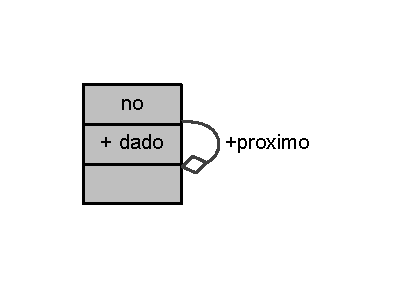
\includegraphics[width=189pt]{structno__coll__graph}
\end{center}
\end{figure}
\subsection*{Data Fields}
\begin{DoxyCompactItemize}
\item 
float \mbox{\hyperlink{structno_a14ddb52e8b1bf70f6adf49d9dc2e23f5}{dado}}
\item 
struct \mbox{\hyperlink{structno}{no}} $\ast$ \mbox{\hyperlink{structno_ac5dac914c4194e089f197231896fa8e0}{proximo}}
\end{DoxyCompactItemize}


\subsection{Detailed Description}


Definition at line 15 of file Calculadora.\+h.



\subsection{Field Documentation}
\mbox{\Hypertarget{structno_a14ddb52e8b1bf70f6adf49d9dc2e23f5}\label{structno_a14ddb52e8b1bf70f6adf49d9dc2e23f5}} 
\index{no@{no}!dado@{dado}}
\index{dado@{dado}!no@{no}}
\subsubsection{\texorpdfstring{dado}{dado}}
{\footnotesize\ttfamily float dado}



Definition at line 16 of file Calculadora.\+h.

\mbox{\Hypertarget{structno_ac5dac914c4194e089f197231896fa8e0}\label{structno_ac5dac914c4194e089f197231896fa8e0}} 
\index{no@{no}!proximo@{proximo}}
\index{proximo@{proximo}!no@{no}}
\subsubsection{\texorpdfstring{proximo}{proximo}}
{\footnotesize\ttfamily struct \mbox{\hyperlink{structno}{no}}$\ast$ proximo}



Definition at line 17 of file Calculadora.\+h.



The documentation for this struct was generated from the following file\+:\begin{DoxyCompactItemize}
\item 
\mbox{\hyperlink{_calculadora_8h}{Calculadora.\+h}}\end{DoxyCompactItemize}

\hypertarget{structno__c}{}\section{no\+\_\+c Struct Reference}
\label{structno__c}\index{no\+\_\+c@{no\+\_\+c}}


{\ttfamily \#include $<$Res\+\_\+exp.\+h$>$}



Collaboration diagram for no\+\_\+c\+:
\nopagebreak
\begin{figure}[H]
\begin{center}
\leavevmode
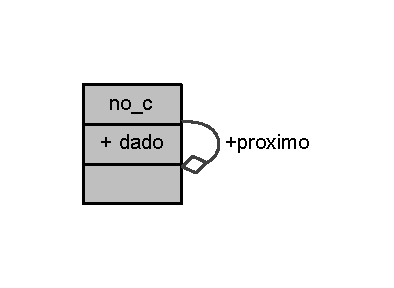
\includegraphics[width=189pt]{structno__c__coll__graph}
\end{center}
\end{figure}
\subsection*{Data Fields}
\begin{DoxyCompactItemize}
\item 
char \mbox{\hyperlink{structno__c_ad8f3850ac3a21b7cd8ed98c5e81ff158}{dado}}
\item 
struct \mbox{\hyperlink{structno__c}{no\+\_\+c}} $\ast$ \mbox{\hyperlink{structno__c_ae377ca56965f4c6b7ce1ed7b465bc7e9}{proximo}}
\end{DoxyCompactItemize}


\subsection{Detailed Description}


Definition at line 15 of file Res\+\_\+exp.\+h.



\subsection{Field Documentation}
\mbox{\Hypertarget{structno__c_ad8f3850ac3a21b7cd8ed98c5e81ff158}\label{structno__c_ad8f3850ac3a21b7cd8ed98c5e81ff158}} 
\index{no\+\_\+c@{no\+\_\+c}!dado@{dado}}
\index{dado@{dado}!no\+\_\+c@{no\+\_\+c}}
\subsubsection{\texorpdfstring{dado}{dado}}
{\footnotesize\ttfamily char dado}



Definition at line 16 of file Res\+\_\+exp.\+h.

\mbox{\Hypertarget{structno__c_ae377ca56965f4c6b7ce1ed7b465bc7e9}\label{structno__c_ae377ca56965f4c6b7ce1ed7b465bc7e9}} 
\index{no\+\_\+c@{no\+\_\+c}!proximo@{proximo}}
\index{proximo@{proximo}!no\+\_\+c@{no\+\_\+c}}
\subsubsection{\texorpdfstring{proximo}{proximo}}
{\footnotesize\ttfamily struct \mbox{\hyperlink{structno__c}{no\+\_\+c}}$\ast$ proximo}



Definition at line 17 of file Res\+\_\+exp.\+h.



The documentation for this struct was generated from the following file\+:\begin{DoxyCompactItemize}
\item 
\mbox{\hyperlink{_res__exp_8h}{Res\+\_\+exp.\+h}}\end{DoxyCompactItemize}

\hypertarget{structt__pilha}{}\section{t\+\_\+pilha Struct Reference}
\label{structt__pilha}\index{t\+\_\+pilha@{t\+\_\+pilha}}


{\ttfamily \#include $<$Calculadora.\+h$>$}



Collaboration diagram for t\+\_\+pilha\+:
\nopagebreak
\begin{figure}[H]
\begin{center}
\leavevmode
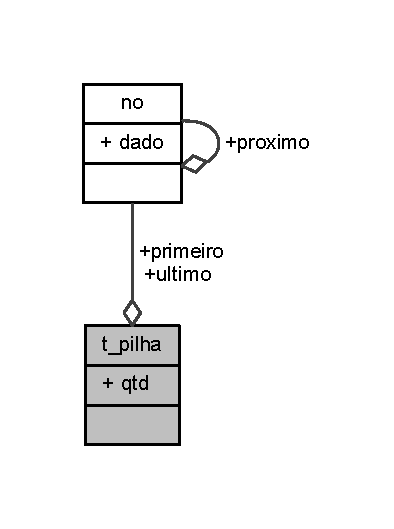
\includegraphics[width=189pt]{structt__pilha__coll__graph}
\end{center}
\end{figure}
\subsection*{Data Fields}
\begin{DoxyCompactItemize}
\item 
\mbox{\hyperlink{_calculadora_8h_a312f04dbe081fc59526dcf1463e3380a}{t\+\_\+no}} $\ast$ \mbox{\hyperlink{structt__pilha_a7934aefd2d1b991f40c0aee790cbe816}{primeiro}}
\item 
\mbox{\hyperlink{_calculadora_8h_a312f04dbe081fc59526dcf1463e3380a}{t\+\_\+no}} $\ast$ \mbox{\hyperlink{structt__pilha_ac877288312a8aa6ba82eed564f15e022}{ultimo}}
\item 
int \mbox{\hyperlink{structt__pilha_ab64e355d6f14927f41266ddfbf88ac91}{qtd}}
\end{DoxyCompactItemize}


\subsection{Detailed Description}


Definition at line 20 of file Calculadora.\+h.



\subsection{Field Documentation}
\mbox{\Hypertarget{structt__pilha_a7934aefd2d1b991f40c0aee790cbe816}\label{structt__pilha_a7934aefd2d1b991f40c0aee790cbe816}} 
\index{t\+\_\+pilha@{t\+\_\+pilha}!primeiro@{primeiro}}
\index{primeiro@{primeiro}!t\+\_\+pilha@{t\+\_\+pilha}}
\subsubsection{\texorpdfstring{primeiro}{primeiro}}
{\footnotesize\ttfamily \mbox{\hyperlink{_calculadora_8h_a312f04dbe081fc59526dcf1463e3380a}{t\+\_\+no}}$\ast$ primeiro}



Definition at line 21 of file Calculadora.\+h.

\mbox{\Hypertarget{structt__pilha_ab64e355d6f14927f41266ddfbf88ac91}\label{structt__pilha_ab64e355d6f14927f41266ddfbf88ac91}} 
\index{t\+\_\+pilha@{t\+\_\+pilha}!qtd@{qtd}}
\index{qtd@{qtd}!t\+\_\+pilha@{t\+\_\+pilha}}
\subsubsection{\texorpdfstring{qtd}{qtd}}
{\footnotesize\ttfamily int qtd}



Definition at line 24 of file Calculadora.\+h.

\mbox{\Hypertarget{structt__pilha_ac877288312a8aa6ba82eed564f15e022}\label{structt__pilha_ac877288312a8aa6ba82eed564f15e022}} 
\index{t\+\_\+pilha@{t\+\_\+pilha}!ultimo@{ultimo}}
\index{ultimo@{ultimo}!t\+\_\+pilha@{t\+\_\+pilha}}
\subsubsection{\texorpdfstring{ultimo}{ultimo}}
{\footnotesize\ttfamily \mbox{\hyperlink{_calculadora_8h_a312f04dbe081fc59526dcf1463e3380a}{t\+\_\+no}}$\ast$ ultimo}



Definition at line 22 of file Calculadora.\+h.



The documentation for this struct was generated from the following file\+:\begin{DoxyCompactItemize}
\item 
\mbox{\hyperlink{_calculadora_8h}{Calculadora.\+h}}\end{DoxyCompactItemize}

\hypertarget{structt__pilha__c}{}\section{t\+\_\+pilha\+\_\+c Struct Reference}
\label{structt__pilha__c}\index{t\+\_\+pilha\+\_\+c@{t\+\_\+pilha\+\_\+c}}


{\ttfamily \#include $<$Res\+\_\+exp.\+h$>$}



Collaboration diagram for t\+\_\+pilha\+\_\+c\+:
\nopagebreak
\begin{figure}[H]
\begin{center}
\leavevmode
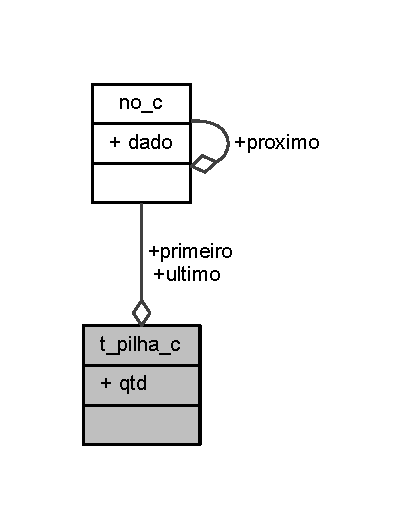
\includegraphics[width=194pt]{structt__pilha__c__coll__graph}
\end{center}
\end{figure}
\subsection*{Data Fields}
\begin{DoxyCompactItemize}
\item 
\mbox{\hyperlink{_res__exp_8h_a49875fde21799e17a8437b9caf0ec7d0}{t\+\_\+no\+\_\+c}} $\ast$ \mbox{\hyperlink{structt__pilha__c_a78b04c824b93d6cb6ce038572bff697b}{primeiro}}
\item 
\mbox{\hyperlink{_res__exp_8h_a49875fde21799e17a8437b9caf0ec7d0}{t\+\_\+no\+\_\+c}} $\ast$ \mbox{\hyperlink{structt__pilha__c_a3bffdac0876453bd94bfcf61880645f4}{ultimo}}
\item 
int \mbox{\hyperlink{structt__pilha__c_ab64e355d6f14927f41266ddfbf88ac91}{qtd}}
\end{DoxyCompactItemize}


\subsection{Detailed Description}


Definition at line 20 of file Res\+\_\+exp.\+h.



\subsection{Field Documentation}
\mbox{\Hypertarget{structt__pilha__c_a78b04c824b93d6cb6ce038572bff697b}\label{structt__pilha__c_a78b04c824b93d6cb6ce038572bff697b}} 
\index{t\+\_\+pilha\+\_\+c@{t\+\_\+pilha\+\_\+c}!primeiro@{primeiro}}
\index{primeiro@{primeiro}!t\+\_\+pilha\+\_\+c@{t\+\_\+pilha\+\_\+c}}
\subsubsection{\texorpdfstring{primeiro}{primeiro}}
{\footnotesize\ttfamily \mbox{\hyperlink{_res__exp_8h_a49875fde21799e17a8437b9caf0ec7d0}{t\+\_\+no\+\_\+c}}$\ast$ primeiro}



Definition at line 21 of file Res\+\_\+exp.\+h.

\mbox{\Hypertarget{structt__pilha__c_ab64e355d6f14927f41266ddfbf88ac91}\label{structt__pilha__c_ab64e355d6f14927f41266ddfbf88ac91}} 
\index{t\+\_\+pilha\+\_\+c@{t\+\_\+pilha\+\_\+c}!qtd@{qtd}}
\index{qtd@{qtd}!t\+\_\+pilha\+\_\+c@{t\+\_\+pilha\+\_\+c}}
\subsubsection{\texorpdfstring{qtd}{qtd}}
{\footnotesize\ttfamily int qtd}



Definition at line 24 of file Res\+\_\+exp.\+h.

\mbox{\Hypertarget{structt__pilha__c_a3bffdac0876453bd94bfcf61880645f4}\label{structt__pilha__c_a3bffdac0876453bd94bfcf61880645f4}} 
\index{t\+\_\+pilha\+\_\+c@{t\+\_\+pilha\+\_\+c}!ultimo@{ultimo}}
\index{ultimo@{ultimo}!t\+\_\+pilha\+\_\+c@{t\+\_\+pilha\+\_\+c}}
\subsubsection{\texorpdfstring{ultimo}{ultimo}}
{\footnotesize\ttfamily \mbox{\hyperlink{_res__exp_8h_a49875fde21799e17a8437b9caf0ec7d0}{t\+\_\+no\+\_\+c}}$\ast$ ultimo}



Definition at line 22 of file Res\+\_\+exp.\+h.



The documentation for this struct was generated from the following file\+:\begin{DoxyCompactItemize}
\item 
\mbox{\hyperlink{_res__exp_8h}{Res\+\_\+exp.\+h}}\end{DoxyCompactItemize}

\chapter{File Documentation}
\hypertarget{_algoritmo__1_8c}{}\section{Algoritmo\+\_\+1.\+c File Reference}
\label{_algoritmo__1_8c}\index{Algoritmo\+\_\+1.\+c@{Algoritmo\+\_\+1.\+c}}
{\ttfamily \#include \char`\"{}Res\+\_\+exp.\+h\char`\"{}}\newline
Include dependency graph for Algoritmo\+\_\+1.\+c\+:
\nopagebreak
\begin{figure}[H]
\begin{center}
\leavevmode
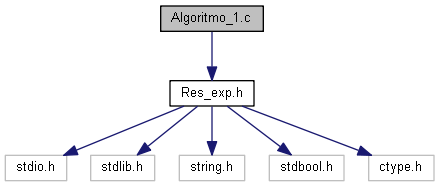
\includegraphics[width=350pt]{_algoritmo__1_8c__incl}
\end{center}
\end{figure}
\subsection*{Functions}
\begin{DoxyCompactItemize}
\item 
int \mbox{\hyperlink{_algoritmo__1_8c_a0450cb0189bf507d2a9f8f057612d795}{valida\+\_\+escopo}} (char $\ast$str, \mbox{\hyperlink{structt__pilha__c}{t\+\_\+pilha\+\_\+c}} $\ast$pilha\+\_\+c)
\end{DoxyCompactItemize}


\subsection{Function Documentation}
\mbox{\Hypertarget{_algoritmo__1_8c_a0450cb0189bf507d2a9f8f057612d795}\label{_algoritmo__1_8c_a0450cb0189bf507d2a9f8f057612d795}} 
\index{Algoritmo\+\_\+1.\+c@{Algoritmo\+\_\+1.\+c}!valida\+\_\+escopo@{valida\+\_\+escopo}}
\index{valida\+\_\+escopo@{valida\+\_\+escopo}!Algoritmo\+\_\+1.\+c@{Algoritmo\+\_\+1.\+c}}
\subsubsection{\texorpdfstring{valida\+\_\+escopo()}{valida\_escopo()}}
{\footnotesize\ttfamily int valida\+\_\+escopo (\begin{DoxyParamCaption}\item[{char $\ast$}]{str,  }\item[{\mbox{\hyperlink{structt__pilha__c}{t\+\_\+pilha\+\_\+c}} $\ast$}]{pilha\+\_\+c }\end{DoxyParamCaption})}



Definition at line 6 of file Algoritmo\+\_\+1.\+c.

Here is the call graph for this function\+:
\nopagebreak
\begin{figure}[H]
\begin{center}
\leavevmode
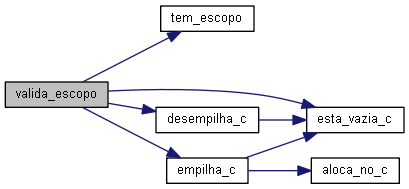
\includegraphics[width=350pt]{_algoritmo__1_8c_a0450cb0189bf507d2a9f8f057612d795_cgraph}
\end{center}
\end{figure}
Here is the caller graph for this function\+:
\nopagebreak
\begin{figure}[H]
\begin{center}
\leavevmode
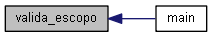
\includegraphics[width=231pt]{_algoritmo__1_8c_a0450cb0189bf507d2a9f8f057612d795_icgraph}
\end{center}
\end{figure}

\hypertarget{_algoritmo__2_8c}{}\section{Algoritmo\+\_\+2.\+c File Reference}
\label{_algoritmo__2_8c}\index{Algoritmo\+\_\+2.\+c@{Algoritmo\+\_\+2.\+c}}
{\ttfamily \#include \char`\"{}Res\+\_\+exp.\+h\char`\"{}}\newline
Include dependency graph for Algoritmo\+\_\+2.\+c\+:
\nopagebreak
\begin{figure}[H]
\begin{center}
\leavevmode
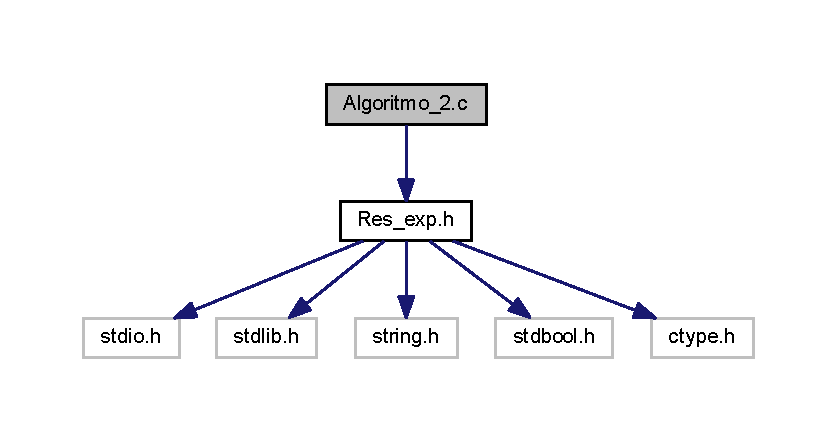
\includegraphics[width=350pt]{_algoritmo__2_8c__incl}
\end{center}
\end{figure}
\subsection*{Functions}
\begin{DoxyCompactItemize}
\item 
int \mbox{\hyperlink{_algoritmo__2_8c_ad0acd78bee8a5b768d35240be8cfb722}{precedencia}} (char c)
\item 
void \mbox{\hyperlink{_algoritmo__2_8c_af2b0252508c5721283cdbdec77164236}{transforma}} (char $\ast$exp\+\_\+infixa, char $\ast$exp\+\_\+posfixa)
\end{DoxyCompactItemize}


\subsection{Function Documentation}
\mbox{\Hypertarget{_algoritmo__2_8c_ad0acd78bee8a5b768d35240be8cfb722}\label{_algoritmo__2_8c_ad0acd78bee8a5b768d35240be8cfb722}} 
\index{Algoritmo\+\_\+2.\+c@{Algoritmo\+\_\+2.\+c}!precedencia@{precedencia}}
\index{precedencia@{precedencia}!Algoritmo\+\_\+2.\+c@{Algoritmo\+\_\+2.\+c}}
\subsubsection{\texorpdfstring{precedencia()}{precedencia()}}
{\footnotesize\ttfamily int precedencia (\begin{DoxyParamCaption}\item[{char}]{c }\end{DoxyParamCaption})}



Definition at line 5 of file Algoritmo\+\_\+2.\+c.

Here is the caller graph for this function\+:
\nopagebreak
\begin{figure}[H]
\begin{center}
\leavevmode
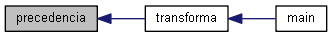
\includegraphics[width=321pt]{_algoritmo__2_8c_ad0acd78bee8a5b768d35240be8cfb722_icgraph}
\end{center}
\end{figure}
\mbox{\Hypertarget{_algoritmo__2_8c_af2b0252508c5721283cdbdec77164236}\label{_algoritmo__2_8c_af2b0252508c5721283cdbdec77164236}} 
\index{Algoritmo\+\_\+2.\+c@{Algoritmo\+\_\+2.\+c}!transforma@{transforma}}
\index{transforma@{transforma}!Algoritmo\+\_\+2.\+c@{Algoritmo\+\_\+2.\+c}}
\subsubsection{\texorpdfstring{transforma()}{transforma()}}
{\footnotesize\ttfamily void transforma (\begin{DoxyParamCaption}\item[{char $\ast$}]{exp\+\_\+infixa,  }\item[{char $\ast$}]{exp\+\_\+posfixa }\end{DoxyParamCaption})}



Definition at line 18 of file Algoritmo\+\_\+2.\+c.

Here is the call graph for this function\+:
\nopagebreak
\begin{figure}[H]
\begin{center}
\leavevmode
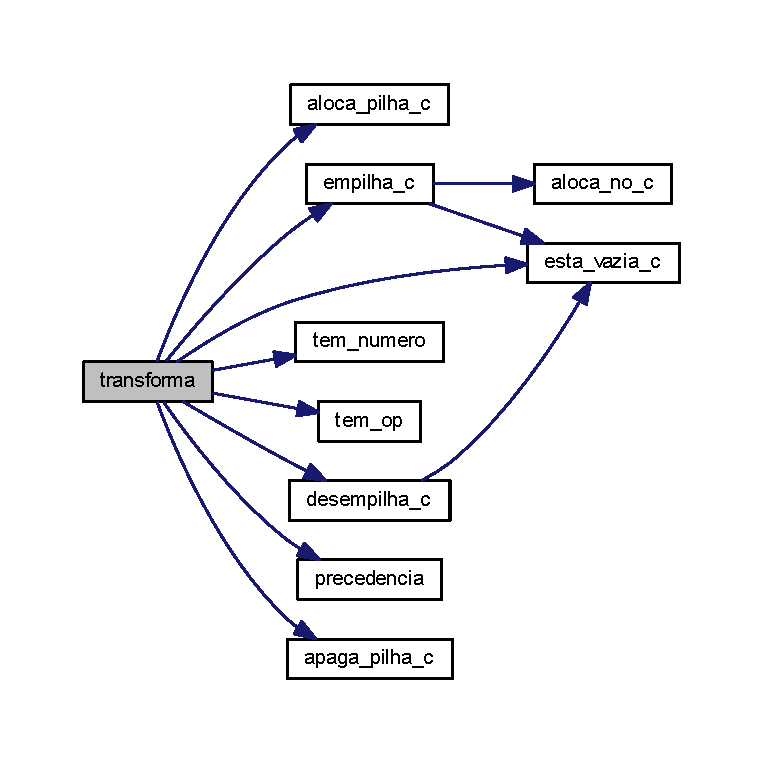
\includegraphics[width=350pt]{_algoritmo__2_8c_af2b0252508c5721283cdbdec77164236_cgraph}
\end{center}
\end{figure}
Here is the caller graph for this function\+:
\nopagebreak
\begin{figure}[H]
\begin{center}
\leavevmode
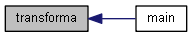
\includegraphics[width=216pt]{_algoritmo__2_8c_af2b0252508c5721283cdbdec77164236_icgraph}
\end{center}
\end{figure}

\hypertarget{_algoritmo__3_8c}{}\section{Algoritmo\+\_\+3.\+c File Reference}
\label{_algoritmo__3_8c}\index{Algoritmo\+\_\+3.\+c@{Algoritmo\+\_\+3.\+c}}
{\ttfamily \#include \char`\"{}Res\+\_\+exp.\+h\char`\"{}}\newline
{\ttfamily \#include \char`\"{}Calculadora.\+h\char`\"{}}\newline
Include dependency graph for Algoritmo\+\_\+3.\+c\+:
\nopagebreak
\begin{figure}[H]
\begin{center}
\leavevmode
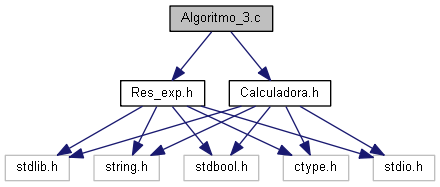
\includegraphics[width=350pt]{_algoritmo__3_8c__incl}
\end{center}
\end{figure}
\subsection*{Functions}
\begin{DoxyCompactItemize}
\item 
float \mbox{\hyperlink{_algoritmo__3_8c_adb2dfa0d22377e798817bd431985a9e3}{resolve\+\_\+posfixa}} (char $\ast$str)
\end{DoxyCompactItemize}


\subsection{Function Documentation}
\mbox{\Hypertarget{_algoritmo__3_8c_adb2dfa0d22377e798817bd431985a9e3}\label{_algoritmo__3_8c_adb2dfa0d22377e798817bd431985a9e3}} 
\index{Algoritmo\+\_\+3.\+c@{Algoritmo\+\_\+3.\+c}!resolve\+\_\+posfixa@{resolve\+\_\+posfixa}}
\index{resolve\+\_\+posfixa@{resolve\+\_\+posfixa}!Algoritmo\+\_\+3.\+c@{Algoritmo\+\_\+3.\+c}}
\subsubsection{\texorpdfstring{resolve\+\_\+posfixa()}{resolve\_posfixa()}}
{\footnotesize\ttfamily float resolve\+\_\+posfixa (\begin{DoxyParamCaption}\item[{char $\ast$}]{str }\end{DoxyParamCaption})}



Definition at line 10 of file Algoritmo\+\_\+3.\+c.

Here is the call graph for this function\+:
\nopagebreak
\begin{figure}[H]
\begin{center}
\leavevmode
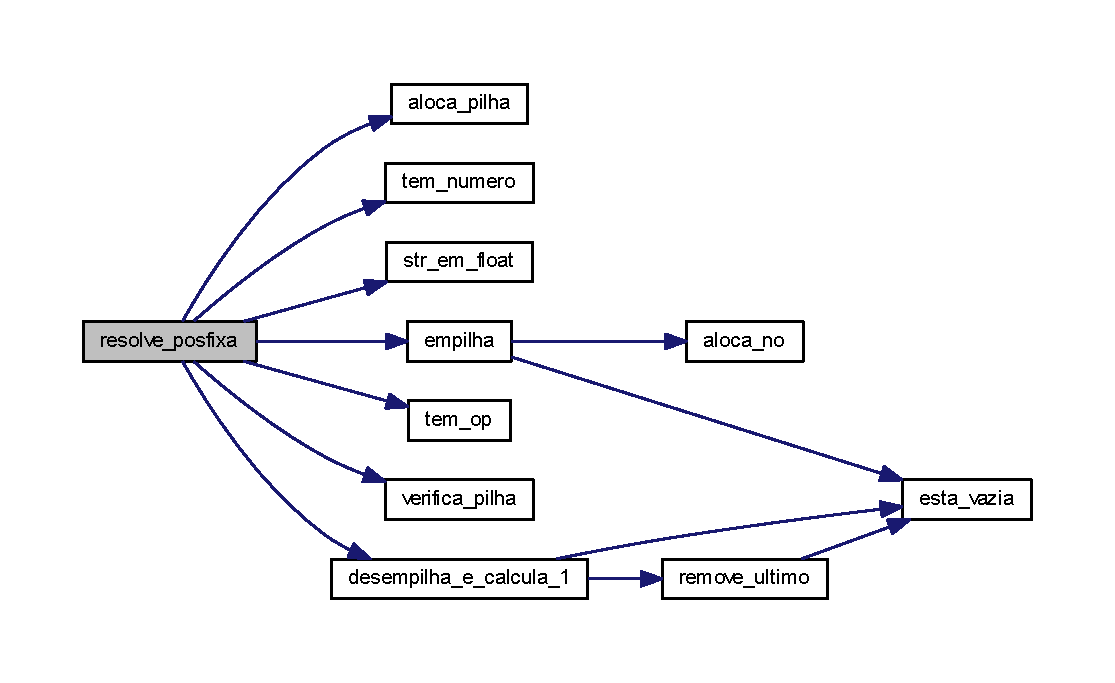
\includegraphics[width=350pt]{_algoritmo__3_8c_adb2dfa0d22377e798817bd431985a9e3_cgraph}
\end{center}
\end{figure}
Here is the caller graph for this function\+:
\nopagebreak
\begin{figure}[H]
\begin{center}
\leavevmode
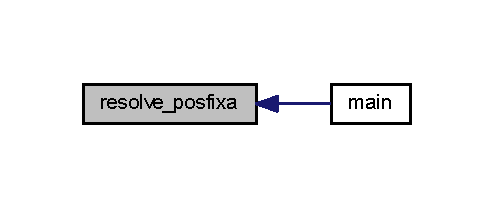
\includegraphics[width=237pt]{_algoritmo__3_8c_adb2dfa0d22377e798817bd431985a9e3_icgraph}
\end{center}
\end{figure}

\hypertarget{_calculadora_8h}{}\section{Calculadora.\+h File Reference}
\label{_calculadora_8h}\index{Calculadora.\+h@{Calculadora.\+h}}
{\ttfamily \#include $<$stdio.\+h$>$}\newline
{\ttfamily \#include $<$stdlib.\+h$>$}\newline
{\ttfamily \#include $<$string.\+h$>$}\newline
{\ttfamily \#include $<$stdbool.\+h$>$}\newline
{\ttfamily \#include $<$ctype.\+h$>$}\newline
Include dependency graph for Calculadora.\+h\+:
\nopagebreak
\begin{figure}[H]
\begin{center}
\leavevmode
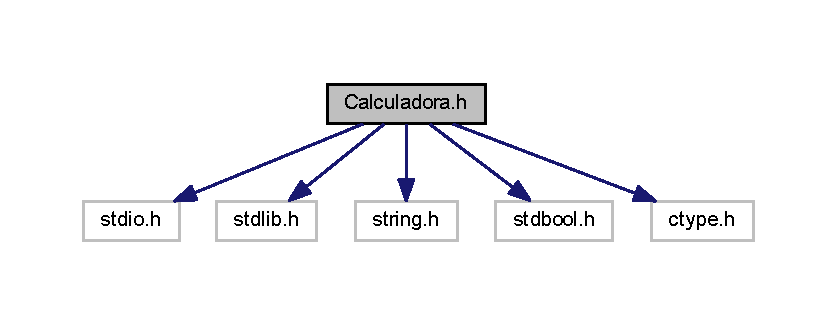
\includegraphics[width=350pt]{_calculadora_8h__incl}
\end{center}
\end{figure}
This graph shows which files directly or indirectly include this file\+:
\nopagebreak
\begin{figure}[H]
\begin{center}
\leavevmode
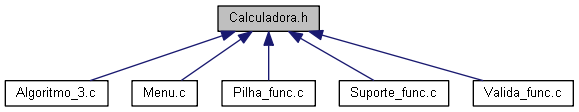
\includegraphics[width=350pt]{_calculadora_8h__dep__incl}
\end{center}
\end{figure}
\subsection*{Data Structures}
\begin{DoxyCompactItemize}
\item 
struct \mbox{\hyperlink{structno}{no}}
\item 
struct \mbox{\hyperlink{structt__pilha}{t\+\_\+pilha}}
\end{DoxyCompactItemize}
\subsection*{Typedefs}
\begin{DoxyCompactItemize}
\item 
typedef struct \mbox{\hyperlink{structno}{no}} \mbox{\hyperlink{_calculadora_8h_a312f04dbe081fc59526dcf1463e3380a}{t\+\_\+no}}
\end{DoxyCompactItemize}
\subsection*{Functions}
\begin{DoxyCompactItemize}
\item 
\mbox{\hyperlink{structt__pilha}{t\+\_\+pilha}} $\ast$ \mbox{\hyperlink{_calculadora_8h_a882b64f15d2cb66bbaeb41a341e71dce}{aloca\+\_\+pilha}} ()
\item 
\mbox{\hyperlink{_calculadora_8h_a312f04dbe081fc59526dcf1463e3380a}{t\+\_\+no}} $\ast$ \mbox{\hyperlink{_calculadora_8h_ade7db9766f53662f025a944b636f4db2}{aloca\+\_\+no}} (float dado)
\item 
int \mbox{\hyperlink{_calculadora_8h_a5705252b26adc92c6a848252ca1790c1}{empilha}} (float dado, \mbox{\hyperlink{structt__pilha}{t\+\_\+pilha}} $\ast$pilha)
\item 
void \mbox{\hyperlink{_calculadora_8h_a7754e1e0150be8a3a784d637ed83a699}{imprime\+\_\+pilha}} (\mbox{\hyperlink{structt__pilha}{t\+\_\+pilha}} $\ast$pilha)
\item 
int \mbox{\hyperlink{_calculadora_8h_adfd347e2b3f0462a4a1bd85e7d033e68}{esta\+\_\+vazia}} (\mbox{\hyperlink{structt__pilha}{t\+\_\+pilha}} $\ast$pilha)
\item 
void \mbox{\hyperlink{_calculadora_8h_a5c485ba4895206b77485169e4d240157}{apaga\+\_\+pilha}} (\mbox{\hyperlink{structt__pilha}{t\+\_\+pilha}} $\ast$pilha)
\item 
int \mbox{\hyperlink{_calculadora_8h_a91d1e173ad5aaecf8348f4429f54c210}{verifica\+\_\+pilha}} (\mbox{\hyperlink{structt__pilha}{t\+\_\+pilha}} $\ast$pilha)
\item 
float \mbox{\hyperlink{_calculadora_8h_a0ce03f1f3ee5207eb5390b0658d1ca69}{desempilha\+\_\+e\+\_\+calcula\+\_\+1}} (char op, \mbox{\hyperlink{structt__pilha}{t\+\_\+pilha}} $\ast$pilha)
\item 
float \mbox{\hyperlink{_calculadora_8h_a23bb611728759ee2acc8523f39b3b34c}{desempilha\+\_\+e\+\_\+calcula\+\_\+2}} (char op, \mbox{\hyperlink{structt__pilha}{t\+\_\+pilha}} $\ast$pilha)
\item 
int \mbox{\hyperlink{_calculadora_8h_a9a11eff29728678483ea05fa1983018c}{remove\+\_\+ultimo}} (\mbox{\hyperlink{structt__pilha}{t\+\_\+pilha}} $\ast$pilha)
\item 
bool \mbox{\hyperlink{_calculadora_8h_ac9a342197c376e2cd018f95b1394618c}{valida\+\_\+str}} (char c)
\item 
bool \mbox{\hyperlink{_calculadora_8h_a938fdba0cc830b48c5d0a85ad31c4bed}{tem\+\_\+char}} (char c)
\item 
bool \mbox{\hyperlink{_calculadora_8h_a6bdb02d6cf0aabad0986f4ed8f5a7056}{tem\+\_\+operador}} (char c)
\item 
int \mbox{\hyperlink{_calculadora_8h_a57b564d2fcef3dd2d88aa2fe653a7771}{check}} (char $\ast$str)
\item 
int \mbox{\hyperlink{_calculadora_8h_a924e3344e312510ba6b0b0a1f63613d9}{copia\+\_\+elemento}} (\mbox{\hyperlink{structt__pilha}{t\+\_\+pilha}} $\ast$pilha)
\item 
void \mbox{\hyperlink{_calculadora_8h_a7b541b1f54cc537f7b83b83b3b746a11}{limpabuffer}} ()
\item 
float \mbox{\hyperlink{_calculadora_8h_aa670fb2fd144dab8265822c4e5f5f09c}{str\+\_\+em\+\_\+float}} (char $\ast$str)
\end{DoxyCompactItemize}


\subsection{Typedef Documentation}
\mbox{\Hypertarget{_calculadora_8h_a312f04dbe081fc59526dcf1463e3380a}\label{_calculadora_8h_a312f04dbe081fc59526dcf1463e3380a}} 
\index{Calculadora.\+h@{Calculadora.\+h}!t\+\_\+no@{t\+\_\+no}}
\index{t\+\_\+no@{t\+\_\+no}!Calculadora.\+h@{Calculadora.\+h}}
\subsubsection{\texorpdfstring{t\+\_\+no}{t\_no}}
{\footnotesize\ttfamily typedef struct \mbox{\hyperlink{structno}{no}} \mbox{\hyperlink{_calculadora_8h_a312f04dbe081fc59526dcf1463e3380a}{t\+\_\+no}}}



\subsection{Function Documentation}
\mbox{\Hypertarget{_calculadora_8h_ade7db9766f53662f025a944b636f4db2}\label{_calculadora_8h_ade7db9766f53662f025a944b636f4db2}} 
\index{Calculadora.\+h@{Calculadora.\+h}!aloca\+\_\+no@{aloca\+\_\+no}}
\index{aloca\+\_\+no@{aloca\+\_\+no}!Calculadora.\+h@{Calculadora.\+h}}
\subsubsection{\texorpdfstring{aloca\+\_\+no()}{aloca\_no()}}
{\footnotesize\ttfamily \mbox{\hyperlink{_calculadora_8h_a312f04dbe081fc59526dcf1463e3380a}{t\+\_\+no}}$\ast$ aloca\+\_\+no (\begin{DoxyParamCaption}\item[{float}]{dado }\end{DoxyParamCaption})}



Definition at line 19 of file Pilha\+\_\+func.\+c.

Here is the caller graph for this function\+:
\nopagebreak
\begin{figure}[H]
\begin{center}
\leavevmode
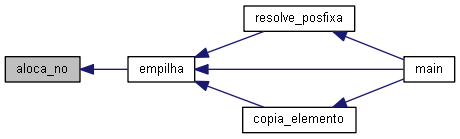
\includegraphics[width=350pt]{_calculadora_8h_ade7db9766f53662f025a944b636f4db2_icgraph}
\end{center}
\end{figure}
\mbox{\Hypertarget{_calculadora_8h_a882b64f15d2cb66bbaeb41a341e71dce}\label{_calculadora_8h_a882b64f15d2cb66bbaeb41a341e71dce}} 
\index{Calculadora.\+h@{Calculadora.\+h}!aloca\+\_\+pilha@{aloca\+\_\+pilha}}
\index{aloca\+\_\+pilha@{aloca\+\_\+pilha}!Calculadora.\+h@{Calculadora.\+h}}
\subsubsection{\texorpdfstring{aloca\+\_\+pilha()}{aloca\_pilha()}}
{\footnotesize\ttfamily \mbox{\hyperlink{structt__pilha}{t\+\_\+pilha}}$\ast$ aloca\+\_\+pilha (\begin{DoxyParamCaption}{ }\end{DoxyParamCaption})}



Definition at line 9 of file Pilha\+\_\+func.\+c.

Here is the caller graph for this function\+:
\nopagebreak
\begin{figure}[H]
\begin{center}
\leavevmode
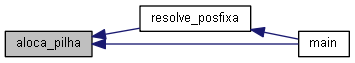
\includegraphics[width=338pt]{_calculadora_8h_a882b64f15d2cb66bbaeb41a341e71dce_icgraph}
\end{center}
\end{figure}
\mbox{\Hypertarget{_calculadora_8h_a5c485ba4895206b77485169e4d240157}\label{_calculadora_8h_a5c485ba4895206b77485169e4d240157}} 
\index{Calculadora.\+h@{Calculadora.\+h}!apaga\+\_\+pilha@{apaga\+\_\+pilha}}
\index{apaga\+\_\+pilha@{apaga\+\_\+pilha}!Calculadora.\+h@{Calculadora.\+h}}
\subsubsection{\texorpdfstring{apaga\+\_\+pilha()}{apaga\_pilha()}}
{\footnotesize\ttfamily void apaga\+\_\+pilha (\begin{DoxyParamCaption}\item[{\mbox{\hyperlink{structt__pilha}{t\+\_\+pilha}} $\ast$}]{pilha }\end{DoxyParamCaption})}



Definition at line 81 of file Pilha\+\_\+func.\+c.

Here is the caller graph for this function\+:
\nopagebreak
\begin{figure}[H]
\begin{center}
\leavevmode
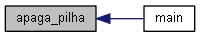
\includegraphics[width=222pt]{_calculadora_8h_a5c485ba4895206b77485169e4d240157_icgraph}
\end{center}
\end{figure}
\mbox{\Hypertarget{_calculadora_8h_a57b564d2fcef3dd2d88aa2fe653a7771}\label{_calculadora_8h_a57b564d2fcef3dd2d88aa2fe653a7771}} 
\index{Calculadora.\+h@{Calculadora.\+h}!check@{check}}
\index{check@{check}!Calculadora.\+h@{Calculadora.\+h}}
\subsubsection{\texorpdfstring{check()}{check()}}
{\footnotesize\ttfamily int check (\begin{DoxyParamCaption}\item[{char $\ast$}]{str }\end{DoxyParamCaption})}



Definition at line 59 of file Valida\+\_\+func.\+c.

Here is the call graph for this function\+:
\nopagebreak
\begin{figure}[H]
\begin{center}
\leavevmode
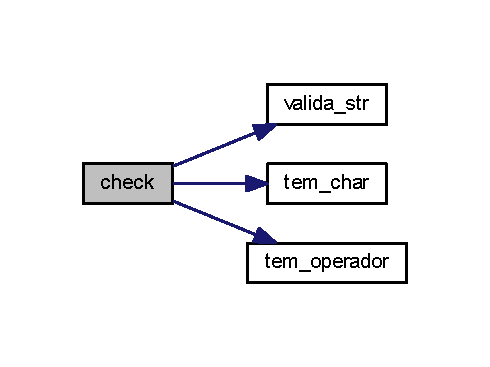
\includegraphics[width=235pt]{_calculadora_8h_a57b564d2fcef3dd2d88aa2fe653a7771_cgraph}
\end{center}
\end{figure}
Here is the caller graph for this function\+:
\nopagebreak
\begin{figure}[H]
\begin{center}
\leavevmode
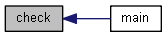
\includegraphics[width=197pt]{_calculadora_8h_a57b564d2fcef3dd2d88aa2fe653a7771_icgraph}
\end{center}
\end{figure}
\mbox{\Hypertarget{_calculadora_8h_a924e3344e312510ba6b0b0a1f63613d9}\label{_calculadora_8h_a924e3344e312510ba6b0b0a1f63613d9}} 
\index{Calculadora.\+h@{Calculadora.\+h}!copia\+\_\+elemento@{copia\+\_\+elemento}}
\index{copia\+\_\+elemento@{copia\+\_\+elemento}!Calculadora.\+h@{Calculadora.\+h}}
\subsubsection{\texorpdfstring{copia\+\_\+elemento()}{copia\_elemento()}}
{\footnotesize\ttfamily int copia\+\_\+elemento (\begin{DoxyParamCaption}\item[{\mbox{\hyperlink{structt__pilha}{t\+\_\+pilha}} $\ast$}]{pilha }\end{DoxyParamCaption})}



Definition at line 7 of file Suporte\+\_\+func.\+c.

Here is the call graph for this function\+:
\nopagebreak
\begin{figure}[H]
\begin{center}
\leavevmode
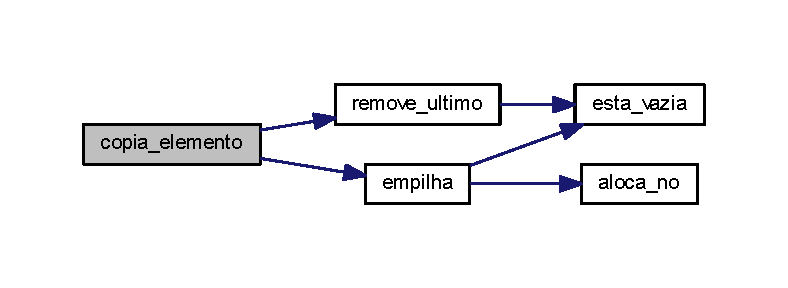
\includegraphics[width=350pt]{_calculadora_8h_a924e3344e312510ba6b0b0a1f63613d9_cgraph}
\end{center}
\end{figure}
Here is the caller graph for this function\+:
\nopagebreak
\begin{figure}[H]
\begin{center}
\leavevmode
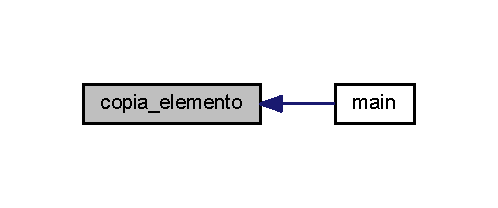
\includegraphics[width=239pt]{_calculadora_8h_a924e3344e312510ba6b0b0a1f63613d9_icgraph}
\end{center}
\end{figure}
\mbox{\Hypertarget{_calculadora_8h_a0ce03f1f3ee5207eb5390b0658d1ca69}\label{_calculadora_8h_a0ce03f1f3ee5207eb5390b0658d1ca69}} 
\index{Calculadora.\+h@{Calculadora.\+h}!desempilha\+\_\+e\+\_\+calcula\+\_\+1@{desempilha\+\_\+e\+\_\+calcula\+\_\+1}}
\index{desempilha\+\_\+e\+\_\+calcula\+\_\+1@{desempilha\+\_\+e\+\_\+calcula\+\_\+1}!Calculadora.\+h@{Calculadora.\+h}}
\subsubsection{\texorpdfstring{desempilha\+\_\+e\+\_\+calcula\+\_\+1()}{desempilha\_e\_calcula\_1()}}
{\footnotesize\ttfamily float desempilha\+\_\+e\+\_\+calcula\+\_\+1 (\begin{DoxyParamCaption}\item[{char}]{op,  }\item[{\mbox{\hyperlink{structt__pilha}{t\+\_\+pilha}} $\ast$}]{pilha }\end{DoxyParamCaption})}



Definition at line 107 of file Pilha\+\_\+func.\+c.

Here is the call graph for this function\+:
\nopagebreak
\begin{figure}[H]
\begin{center}
\leavevmode
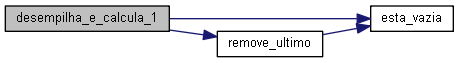
\includegraphics[width=350pt]{_calculadora_8h_a0ce03f1f3ee5207eb5390b0658d1ca69_cgraph}
\end{center}
\end{figure}
Here is the caller graph for this function\+:
\nopagebreak
\begin{figure}[H]
\begin{center}
\leavevmode
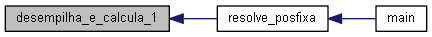
\includegraphics[width=350pt]{_calculadora_8h_a0ce03f1f3ee5207eb5390b0658d1ca69_icgraph}
\end{center}
\end{figure}
\mbox{\Hypertarget{_calculadora_8h_a23bb611728759ee2acc8523f39b3b34c}\label{_calculadora_8h_a23bb611728759ee2acc8523f39b3b34c}} 
\index{Calculadora.\+h@{Calculadora.\+h}!desempilha\+\_\+e\+\_\+calcula\+\_\+2@{desempilha\+\_\+e\+\_\+calcula\+\_\+2}}
\index{desempilha\+\_\+e\+\_\+calcula\+\_\+2@{desempilha\+\_\+e\+\_\+calcula\+\_\+2}!Calculadora.\+h@{Calculadora.\+h}}
\subsubsection{\texorpdfstring{desempilha\+\_\+e\+\_\+calcula\+\_\+2()}{desempilha\_e\_calcula\_2()}}
{\footnotesize\ttfamily float desempilha\+\_\+e\+\_\+calcula\+\_\+2 (\begin{DoxyParamCaption}\item[{char}]{op,  }\item[{\mbox{\hyperlink{structt__pilha}{t\+\_\+pilha}} $\ast$}]{pilha }\end{DoxyParamCaption})}



Definition at line 164 of file Pilha\+\_\+func.\+c.

Here is the call graph for this function\+:
\nopagebreak
\begin{figure}[H]
\begin{center}
\leavevmode
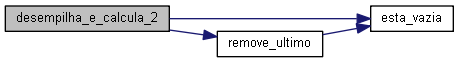
\includegraphics[width=350pt]{_calculadora_8h_a23bb611728759ee2acc8523f39b3b34c_cgraph}
\end{center}
\end{figure}
Here is the caller graph for this function\+:
\nopagebreak
\begin{figure}[H]
\begin{center}
\leavevmode
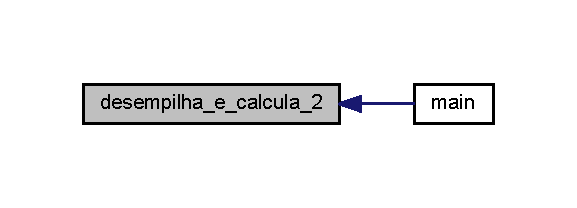
\includegraphics[width=277pt]{_calculadora_8h_a23bb611728759ee2acc8523f39b3b34c_icgraph}
\end{center}
\end{figure}
\mbox{\Hypertarget{_calculadora_8h_a5705252b26adc92c6a848252ca1790c1}\label{_calculadora_8h_a5705252b26adc92c6a848252ca1790c1}} 
\index{Calculadora.\+h@{Calculadora.\+h}!empilha@{empilha}}
\index{empilha@{empilha}!Calculadora.\+h@{Calculadora.\+h}}
\subsubsection{\texorpdfstring{empilha()}{empilha()}}
{\footnotesize\ttfamily int empilha (\begin{DoxyParamCaption}\item[{float}]{dado,  }\item[{\mbox{\hyperlink{structt__pilha}{t\+\_\+pilha}} $\ast$}]{pilha }\end{DoxyParamCaption})}



Definition at line 34 of file Pilha\+\_\+func.\+c.

Here is the call graph for this function\+:
\nopagebreak
\begin{figure}[H]
\begin{center}
\leavevmode
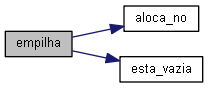
\includegraphics[width=228pt]{_calculadora_8h_a5705252b26adc92c6a848252ca1790c1_cgraph}
\end{center}
\end{figure}
Here is the caller graph for this function\+:
\nopagebreak
\begin{figure}[H]
\begin{center}
\leavevmode
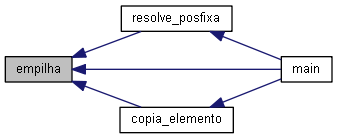
\includegraphics[width=325pt]{_calculadora_8h_a5705252b26adc92c6a848252ca1790c1_icgraph}
\end{center}
\end{figure}
\mbox{\Hypertarget{_calculadora_8h_adfd347e2b3f0462a4a1bd85e7d033e68}\label{_calculadora_8h_adfd347e2b3f0462a4a1bd85e7d033e68}} 
\index{Calculadora.\+h@{Calculadora.\+h}!esta\+\_\+vazia@{esta\+\_\+vazia}}
\index{esta\+\_\+vazia@{esta\+\_\+vazia}!Calculadora.\+h@{Calculadora.\+h}}
\subsubsection{\texorpdfstring{esta\+\_\+vazia()}{esta\_vazia()}}
{\footnotesize\ttfamily int esta\+\_\+vazia (\begin{DoxyParamCaption}\item[{\mbox{\hyperlink{structt__pilha}{t\+\_\+pilha}} $\ast$}]{pilha }\end{DoxyParamCaption})}



Definition at line 76 of file Pilha\+\_\+func.\+c.

Here is the caller graph for this function\+:
\nopagebreak
\begin{figure}[H]
\begin{center}
\leavevmode
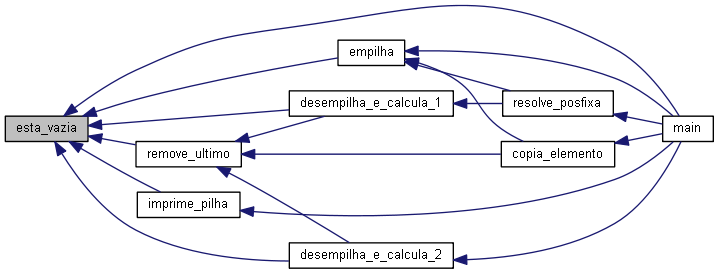
\includegraphics[width=350pt]{_calculadora_8h_adfd347e2b3f0462a4a1bd85e7d033e68_icgraph}
\end{center}
\end{figure}
\mbox{\Hypertarget{_calculadora_8h_a7754e1e0150be8a3a784d637ed83a699}\label{_calculadora_8h_a7754e1e0150be8a3a784d637ed83a699}} 
\index{Calculadora.\+h@{Calculadora.\+h}!imprime\+\_\+pilha@{imprime\+\_\+pilha}}
\index{imprime\+\_\+pilha@{imprime\+\_\+pilha}!Calculadora.\+h@{Calculadora.\+h}}
\subsubsection{\texorpdfstring{imprime\+\_\+pilha()}{imprime\_pilha()}}
{\footnotesize\ttfamily void imprime\+\_\+pilha (\begin{DoxyParamCaption}\item[{\mbox{\hyperlink{structt__pilha}{t\+\_\+pilha}} $\ast$}]{pilha }\end{DoxyParamCaption})}



Definition at line 60 of file Pilha\+\_\+func.\+c.

Here is the call graph for this function\+:
\nopagebreak
\begin{figure}[H]
\begin{center}
\leavevmode
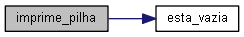
\includegraphics[width=255pt]{_calculadora_8h_a7754e1e0150be8a3a784d637ed83a699_cgraph}
\end{center}
\end{figure}
Here is the caller graph for this function\+:
\nopagebreak
\begin{figure}[H]
\begin{center}
\leavevmode
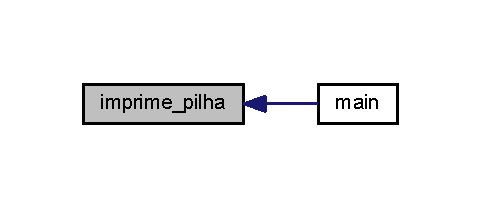
\includegraphics[width=231pt]{_calculadora_8h_a7754e1e0150be8a3a784d637ed83a699_icgraph}
\end{center}
\end{figure}
\mbox{\Hypertarget{_calculadora_8h_a7b541b1f54cc537f7b83b83b3b746a11}\label{_calculadora_8h_a7b541b1f54cc537f7b83b83b3b746a11}} 
\index{Calculadora.\+h@{Calculadora.\+h}!limpabuffer@{limpabuffer}}
\index{limpabuffer@{limpabuffer}!Calculadora.\+h@{Calculadora.\+h}}
\subsubsection{\texorpdfstring{limpabuffer()}{limpabuffer()}}
{\footnotesize\ttfamily void limpabuffer (\begin{DoxyParamCaption}{ }\end{DoxyParamCaption})}



Definition at line 33 of file Suporte\+\_\+func.\+c.

Here is the caller graph for this function\+:
\nopagebreak
\begin{figure}[H]
\begin{center}
\leavevmode
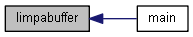
\includegraphics[width=217pt]{_calculadora_8h_a7b541b1f54cc537f7b83b83b3b746a11_icgraph}
\end{center}
\end{figure}
\mbox{\Hypertarget{_calculadora_8h_a9a11eff29728678483ea05fa1983018c}\label{_calculadora_8h_a9a11eff29728678483ea05fa1983018c}} 
\index{Calculadora.\+h@{Calculadora.\+h}!remove\+\_\+ultimo@{remove\+\_\+ultimo}}
\index{remove\+\_\+ultimo@{remove\+\_\+ultimo}!Calculadora.\+h@{Calculadora.\+h}}
\subsubsection{\texorpdfstring{remove\+\_\+ultimo()}{remove\_ultimo()}}
{\footnotesize\ttfamily int remove\+\_\+ultimo (\begin{DoxyParamCaption}\item[{\mbox{\hyperlink{structt__pilha}{t\+\_\+pilha}} $\ast$}]{pilha }\end{DoxyParamCaption})}



Definition at line 221 of file Pilha\+\_\+func.\+c.

Here is the call graph for this function\+:
\nopagebreak
\begin{figure}[H]
\begin{center}
\leavevmode
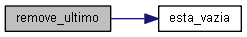
\includegraphics[width=257pt]{_calculadora_8h_a9a11eff29728678483ea05fa1983018c_cgraph}
\end{center}
\end{figure}
Here is the caller graph for this function\+:
\nopagebreak
\begin{figure}[H]
\begin{center}
\leavevmode
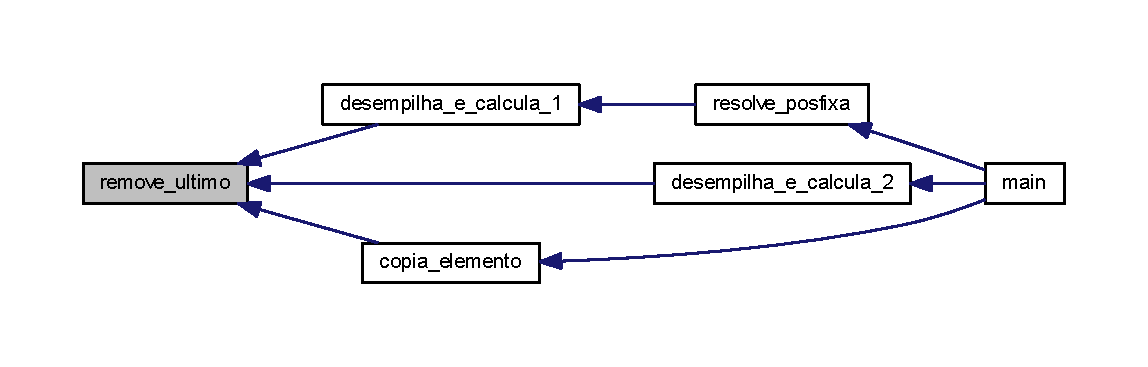
\includegraphics[width=350pt]{_calculadora_8h_a9a11eff29728678483ea05fa1983018c_icgraph}
\end{center}
\end{figure}
\mbox{\Hypertarget{_calculadora_8h_aa670fb2fd144dab8265822c4e5f5f09c}\label{_calculadora_8h_aa670fb2fd144dab8265822c4e5f5f09c}} 
\index{Calculadora.\+h@{Calculadora.\+h}!str\+\_\+em\+\_\+float@{str\+\_\+em\+\_\+float}}
\index{str\+\_\+em\+\_\+float@{str\+\_\+em\+\_\+float}!Calculadora.\+h@{Calculadora.\+h}}
\subsubsection{\texorpdfstring{str\+\_\+em\+\_\+float()}{str\_em\_float()}}
{\footnotesize\ttfamily float str\+\_\+em\+\_\+float (\begin{DoxyParamCaption}\item[{char $\ast$}]{str }\end{DoxyParamCaption})}



Definition at line 39 of file Suporte\+\_\+func.\+c.

Here is the caller graph for this function\+:
\nopagebreak
\begin{figure}[H]
\begin{center}
\leavevmode
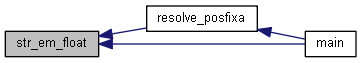
\includegraphics[width=343pt]{_calculadora_8h_aa670fb2fd144dab8265822c4e5f5f09c_icgraph}
\end{center}
\end{figure}
\mbox{\Hypertarget{_calculadora_8h_a938fdba0cc830b48c5d0a85ad31c4bed}\label{_calculadora_8h_a938fdba0cc830b48c5d0a85ad31c4bed}} 
\index{Calculadora.\+h@{Calculadora.\+h}!tem\+\_\+char@{tem\+\_\+char}}
\index{tem\+\_\+char@{tem\+\_\+char}!Calculadora.\+h@{Calculadora.\+h}}
\subsubsection{\texorpdfstring{tem\+\_\+char()}{tem\_char()}}
{\footnotesize\ttfamily bool tem\+\_\+char (\begin{DoxyParamCaption}\item[{char}]{c }\end{DoxyParamCaption})}



Definition at line 32 of file Valida\+\_\+func.\+c.

Here is the caller graph for this function\+:
\nopagebreak
\begin{figure}[H]
\begin{center}
\leavevmode
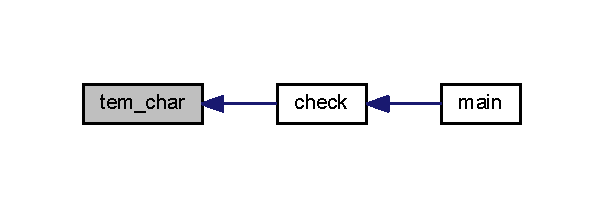
\includegraphics[width=290pt]{_calculadora_8h_a938fdba0cc830b48c5d0a85ad31c4bed_icgraph}
\end{center}
\end{figure}
\mbox{\Hypertarget{_calculadora_8h_a6bdb02d6cf0aabad0986f4ed8f5a7056}\label{_calculadora_8h_a6bdb02d6cf0aabad0986f4ed8f5a7056}} 
\index{Calculadora.\+h@{Calculadora.\+h}!tem\+\_\+operador@{tem\+\_\+operador}}
\index{tem\+\_\+operador@{tem\+\_\+operador}!Calculadora.\+h@{Calculadora.\+h}}
\subsubsection{\texorpdfstring{tem\+\_\+operador()}{tem\_operador()}}
{\footnotesize\ttfamily bool tem\+\_\+operador (\begin{DoxyParamCaption}\item[{char}]{c }\end{DoxyParamCaption})}



Definition at line 46 of file Valida\+\_\+func.\+c.

Here is the caller graph for this function\+:
\nopagebreak
\begin{figure}[H]
\begin{center}
\leavevmode
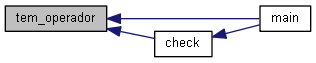
\includegraphics[width=309pt]{_calculadora_8h_a6bdb02d6cf0aabad0986f4ed8f5a7056_icgraph}
\end{center}
\end{figure}
\mbox{\Hypertarget{_calculadora_8h_ac9a342197c376e2cd018f95b1394618c}\label{_calculadora_8h_ac9a342197c376e2cd018f95b1394618c}} 
\index{Calculadora.\+h@{Calculadora.\+h}!valida\+\_\+str@{valida\+\_\+str}}
\index{valida\+\_\+str@{valida\+\_\+str}!Calculadora.\+h@{Calculadora.\+h}}
\subsubsection{\texorpdfstring{valida\+\_\+str()}{valida\_str()}}
{\footnotesize\ttfamily bool valida\+\_\+str (\begin{DoxyParamCaption}\item[{char}]{c }\end{DoxyParamCaption})}



Definition at line 7 of file Valida\+\_\+func.\+c.

Here is the caller graph for this function\+:
\nopagebreak
\begin{figure}[H]
\begin{center}
\leavevmode
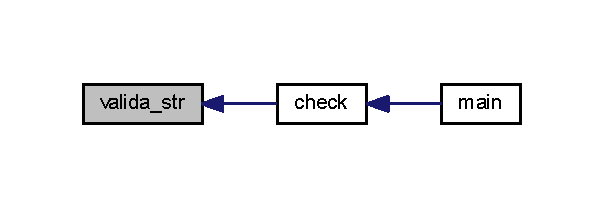
\includegraphics[width=290pt]{_calculadora_8h_ac9a342197c376e2cd018f95b1394618c_icgraph}
\end{center}
\end{figure}
\mbox{\Hypertarget{_calculadora_8h_a91d1e173ad5aaecf8348f4429f54c210}\label{_calculadora_8h_a91d1e173ad5aaecf8348f4429f54c210}} 
\index{Calculadora.\+h@{Calculadora.\+h}!verifica\+\_\+pilha@{verifica\+\_\+pilha}}
\index{verifica\+\_\+pilha@{verifica\+\_\+pilha}!Calculadora.\+h@{Calculadora.\+h}}
\subsubsection{\texorpdfstring{verifica\+\_\+pilha()}{verifica\_pilha()}}
{\footnotesize\ttfamily int verifica\+\_\+pilha (\begin{DoxyParamCaption}\item[{\mbox{\hyperlink{structt__pilha}{t\+\_\+pilha}} $\ast$}]{pilha }\end{DoxyParamCaption})}



Definition at line 97 of file Pilha\+\_\+func.\+c.

Here is the caller graph for this function\+:
\nopagebreak
\begin{figure}[H]
\begin{center}
\leavevmode
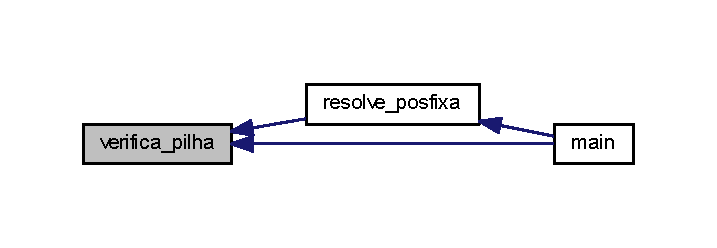
\includegraphics[width=344pt]{_calculadora_8h_a91d1e173ad5aaecf8348f4429f54c210_icgraph}
\end{center}
\end{figure}

\hypertarget{_menu_8c}{}\section{Menu.\+c File Reference}
\label{_menu_8c}\index{Menu.\+c@{Menu.\+c}}
{\ttfamily \#include \char`\"{}Calculadora.\+h\char`\"{}}\newline
{\ttfamily \#include \char`\"{}Res\+\_\+exp.\+h\char`\"{}}\newline
Include dependency graph for Menu.\+c\+:
\nopagebreak
\begin{figure}[H]
\begin{center}
\leavevmode
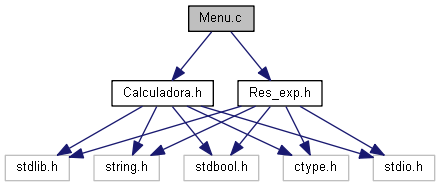
\includegraphics[width=350pt]{_menu_8c__incl}
\end{center}
\end{figure}
\subsection*{Functions}
\begin{DoxyCompactItemize}
\item 
int \mbox{\hyperlink{_menu_8c_ae66f6b31b5ad750f1fe042a706a4e3d4}{main}} ()
\end{DoxyCompactItemize}


\subsection{Function Documentation}
\mbox{\Hypertarget{_menu_8c_ae66f6b31b5ad750f1fe042a706a4e3d4}\label{_menu_8c_ae66f6b31b5ad750f1fe042a706a4e3d4}} 
\index{Menu.\+c@{Menu.\+c}!main@{main}}
\index{main@{main}!Menu.\+c@{Menu.\+c}}
\subsubsection{\texorpdfstring{main()}{main()}}
{\footnotesize\ttfamily int main (\begin{DoxyParamCaption}{ }\end{DoxyParamCaption})}



Definition at line 7 of file Menu.\+c.

Here is the call graph for this function\+:
\nopagebreak
\begin{figure}[H]
\begin{center}
\leavevmode
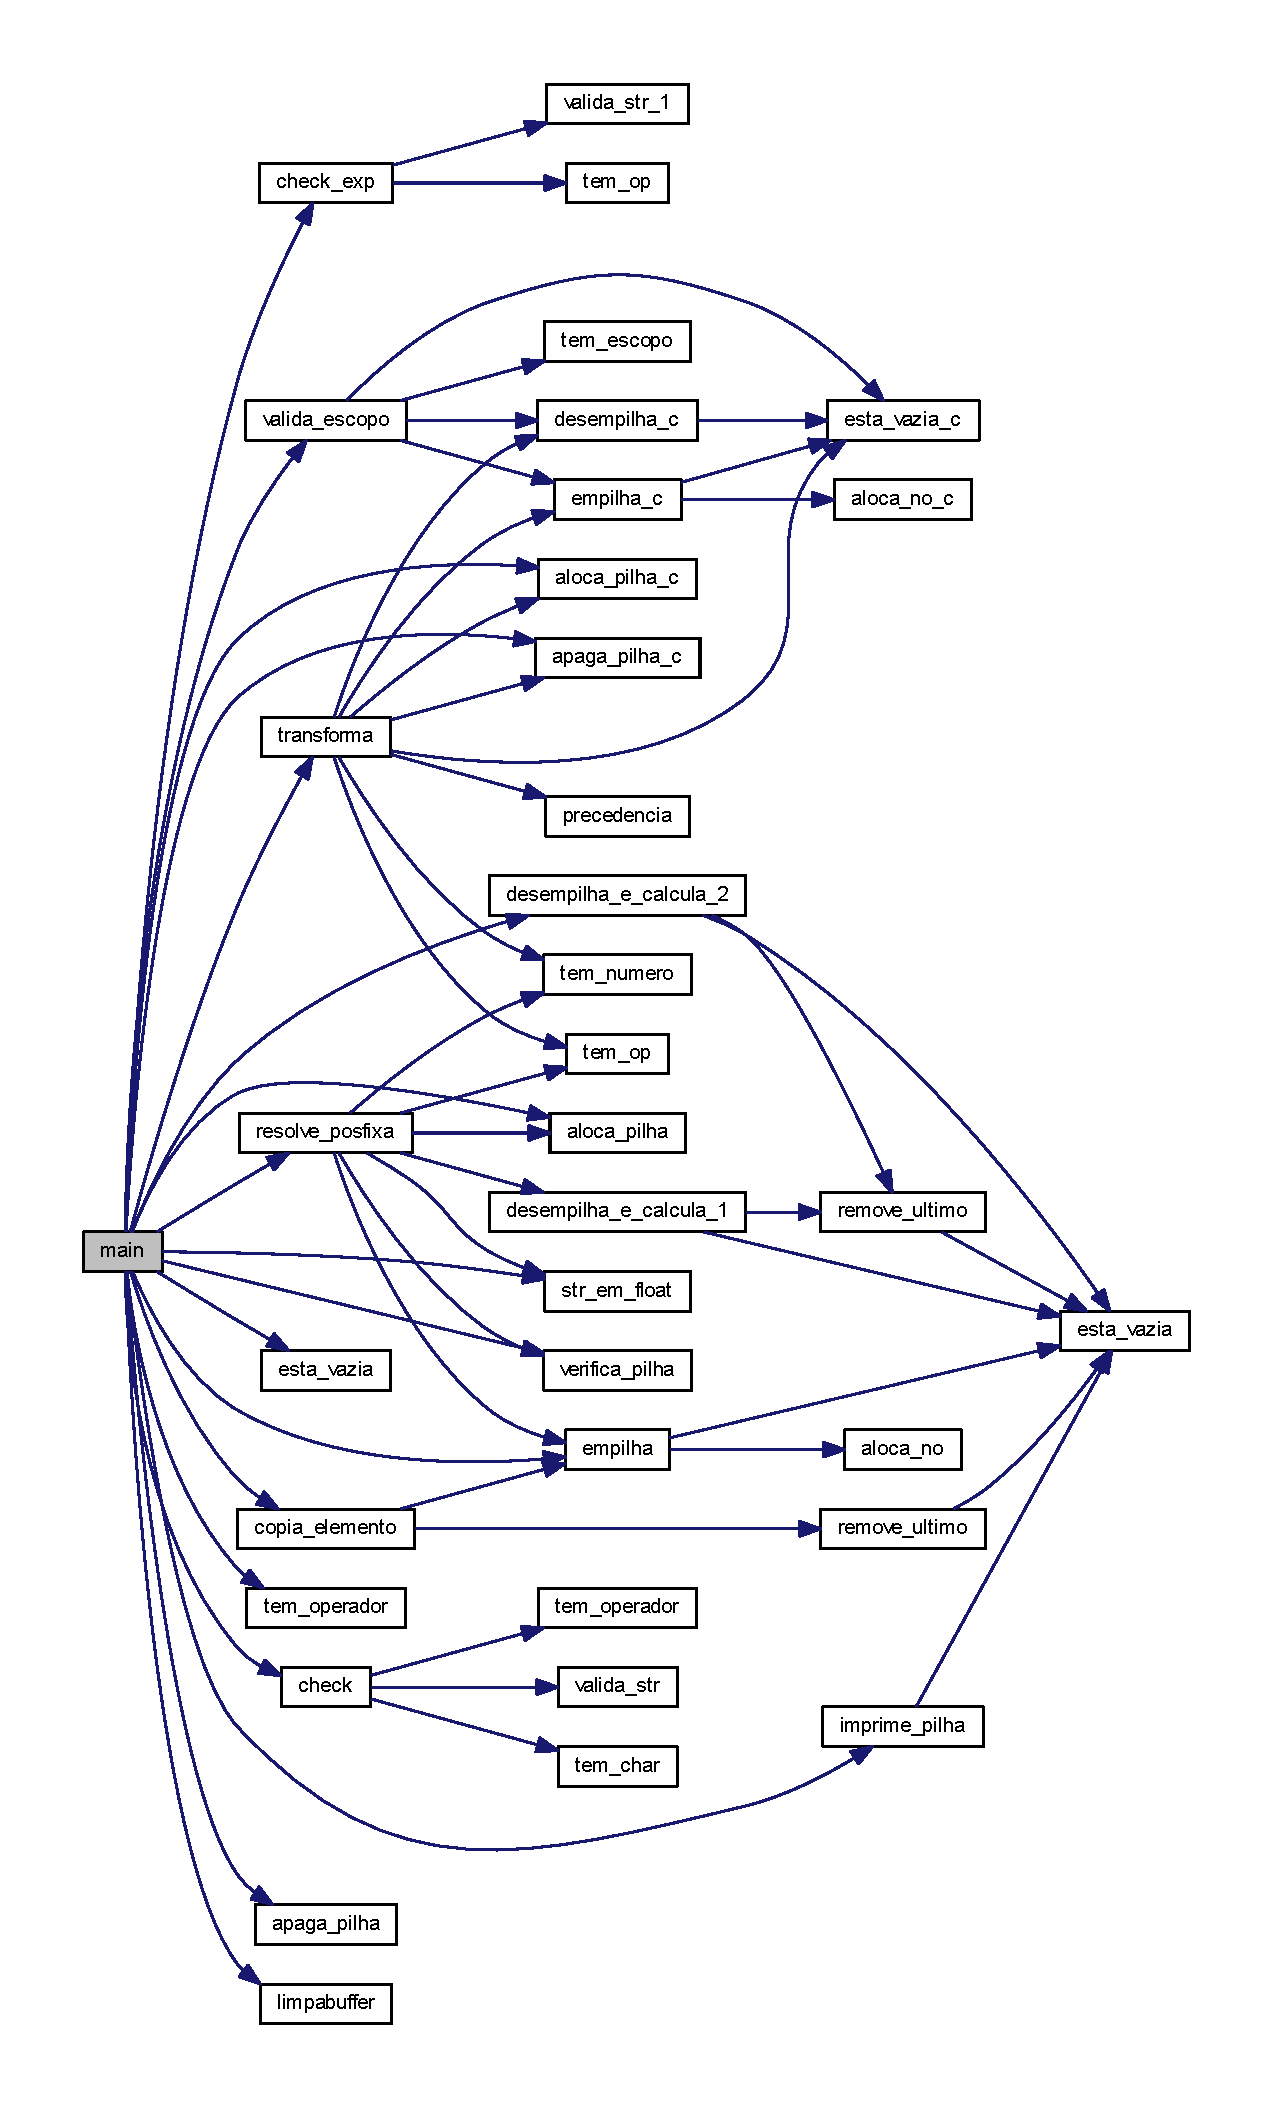
\includegraphics[height=550pt]{_menu_8c_ae66f6b31b5ad750f1fe042a706a4e3d4_cgraph}
\end{center}
\end{figure}

\hypertarget{_pilha__c__func_8c}{}\section{Pilha\+\_\+c\+\_\+func.\+c File Reference}
\label{_pilha__c__func_8c}\index{Pilha\+\_\+c\+\_\+func.\+c@{Pilha\+\_\+c\+\_\+func.\+c}}
{\ttfamily \#include \char`\"{}Res\+\_\+exp.\+h\char`\"{}}\newline
Include dependency graph for Pilha\+\_\+c\+\_\+func.\+c\+:
\nopagebreak
\begin{figure}[H]
\begin{center}
\leavevmode
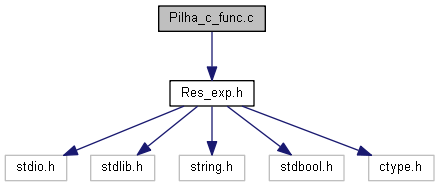
\includegraphics[width=350pt]{_pilha__c__func_8c__incl}
\end{center}
\end{figure}
\subsection*{Functions}
\begin{DoxyCompactItemize}
\item 
\mbox{\hyperlink{structt__pilha__c}{t\+\_\+pilha\+\_\+c}} $\ast$ \mbox{\hyperlink{_pilha__c__func_8c_ae39ed0ad591d07a0c9fde8b10b285b43}{aloca\+\_\+pilha\+\_\+c}} ()
\item 
\mbox{\hyperlink{_res__exp_8h_a49875fde21799e17a8437b9caf0ec7d0}{t\+\_\+no\+\_\+c}} $\ast$ \mbox{\hyperlink{_pilha__c__func_8c_ae39c6a9b3cac787d0587ac6168ede0f4}{aloca\+\_\+no\+\_\+c}} (char dado)
\item 
int \mbox{\hyperlink{_pilha__c__func_8c_a6b3dbcbb549fcd84a7e5aa1207dbc63c}{empilha\+\_\+c}} (char dado, \mbox{\hyperlink{structt__pilha__c}{t\+\_\+pilha\+\_\+c}} $\ast$pilha\+\_\+c)
\item 
char \mbox{\hyperlink{_pilha__c__func_8c_a53f4387852673f6e27870e3f05408aeb}{desempilha\+\_\+c}} (\mbox{\hyperlink{structt__pilha__c}{t\+\_\+pilha\+\_\+c}} $\ast$pilha\+\_\+c)
\item 
int \mbox{\hyperlink{_pilha__c__func_8c_a28d30a9fcbf08a1f95ac47993a89acfc}{esta\+\_\+vazia\+\_\+c}} (\mbox{\hyperlink{structt__pilha__c}{t\+\_\+pilha\+\_\+c}} $\ast$pilha\+\_\+c)
\item 
void \mbox{\hyperlink{_pilha__c__func_8c_aeb21de9a00099b2715658d50ec54c6e5}{apaga\+\_\+pilha\+\_\+c}} (\mbox{\hyperlink{structt__pilha__c}{t\+\_\+pilha\+\_\+c}} $\ast$pilha\+\_\+c)
\end{DoxyCompactItemize}


\subsection{Function Documentation}
\mbox{\Hypertarget{_pilha__c__func_8c_ae39c6a9b3cac787d0587ac6168ede0f4}\label{_pilha__c__func_8c_ae39c6a9b3cac787d0587ac6168ede0f4}} 
\index{Pilha\+\_\+c\+\_\+func.\+c@{Pilha\+\_\+c\+\_\+func.\+c}!aloca\+\_\+no\+\_\+c@{aloca\+\_\+no\+\_\+c}}
\index{aloca\+\_\+no\+\_\+c@{aloca\+\_\+no\+\_\+c}!Pilha\+\_\+c\+\_\+func.\+c@{Pilha\+\_\+c\+\_\+func.\+c}}
\subsubsection{\texorpdfstring{aloca\+\_\+no\+\_\+c()}{aloca\_no\_c()}}
{\footnotesize\ttfamily \mbox{\hyperlink{_res__exp_8h_a49875fde21799e17a8437b9caf0ec7d0}{t\+\_\+no\+\_\+c}}$\ast$ aloca\+\_\+no\+\_\+c (\begin{DoxyParamCaption}\item[{char}]{dado }\end{DoxyParamCaption})}



Definition at line 20 of file Pilha\+\_\+c\+\_\+func.\+c.

Here is the caller graph for this function\+:
\nopagebreak
\begin{figure}[H]
\begin{center}
\leavevmode
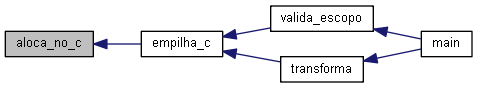
\includegraphics[width=350pt]{_pilha__c__func_8c_ae39c6a9b3cac787d0587ac6168ede0f4_icgraph}
\end{center}
\end{figure}
\mbox{\Hypertarget{_pilha__c__func_8c_ae39ed0ad591d07a0c9fde8b10b285b43}\label{_pilha__c__func_8c_ae39ed0ad591d07a0c9fde8b10b285b43}} 
\index{Pilha\+\_\+c\+\_\+func.\+c@{Pilha\+\_\+c\+\_\+func.\+c}!aloca\+\_\+pilha\+\_\+c@{aloca\+\_\+pilha\+\_\+c}}
\index{aloca\+\_\+pilha\+\_\+c@{aloca\+\_\+pilha\+\_\+c}!Pilha\+\_\+c\+\_\+func.\+c@{Pilha\+\_\+c\+\_\+func.\+c}}
\subsubsection{\texorpdfstring{aloca\+\_\+pilha\+\_\+c()}{aloca\_pilha\_c()}}
{\footnotesize\ttfamily \mbox{\hyperlink{structt__pilha__c}{t\+\_\+pilha\+\_\+c}}$\ast$ aloca\+\_\+pilha\+\_\+c (\begin{DoxyParamCaption}{ }\end{DoxyParamCaption})}



Definition at line 9 of file Pilha\+\_\+c\+\_\+func.\+c.

Here is the caller graph for this function\+:
\nopagebreak
\begin{figure}[H]
\begin{center}
\leavevmode
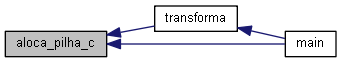
\includegraphics[width=328pt]{_pilha__c__func_8c_ae39ed0ad591d07a0c9fde8b10b285b43_icgraph}
\end{center}
\end{figure}
\mbox{\Hypertarget{_pilha__c__func_8c_aeb21de9a00099b2715658d50ec54c6e5}\label{_pilha__c__func_8c_aeb21de9a00099b2715658d50ec54c6e5}} 
\index{Pilha\+\_\+c\+\_\+func.\+c@{Pilha\+\_\+c\+\_\+func.\+c}!apaga\+\_\+pilha\+\_\+c@{apaga\+\_\+pilha\+\_\+c}}
\index{apaga\+\_\+pilha\+\_\+c@{apaga\+\_\+pilha\+\_\+c}!Pilha\+\_\+c\+\_\+func.\+c@{Pilha\+\_\+c\+\_\+func.\+c}}
\subsubsection{\texorpdfstring{apaga\+\_\+pilha\+\_\+c()}{apaga\_pilha\_c()}}
{\footnotesize\ttfamily void apaga\+\_\+pilha\+\_\+c (\begin{DoxyParamCaption}\item[{\mbox{\hyperlink{structt__pilha__c}{t\+\_\+pilha\+\_\+c}} $\ast$}]{pilha\+\_\+c }\end{DoxyParamCaption})}



Definition at line 107 of file Pilha\+\_\+c\+\_\+func.\+c.

Here is the caller graph for this function\+:
\nopagebreak
\begin{figure}[H]
\begin{center}
\leavevmode
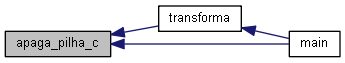
\includegraphics[width=331pt]{_pilha__c__func_8c_aeb21de9a00099b2715658d50ec54c6e5_icgraph}
\end{center}
\end{figure}
\mbox{\Hypertarget{_pilha__c__func_8c_a53f4387852673f6e27870e3f05408aeb}\label{_pilha__c__func_8c_a53f4387852673f6e27870e3f05408aeb}} 
\index{Pilha\+\_\+c\+\_\+func.\+c@{Pilha\+\_\+c\+\_\+func.\+c}!desempilha\+\_\+c@{desempilha\+\_\+c}}
\index{desempilha\+\_\+c@{desempilha\+\_\+c}!Pilha\+\_\+c\+\_\+func.\+c@{Pilha\+\_\+c\+\_\+func.\+c}}
\subsubsection{\texorpdfstring{desempilha\+\_\+c()}{desempilha\_c()}}
{\footnotesize\ttfamily char desempilha\+\_\+c (\begin{DoxyParamCaption}\item[{\mbox{\hyperlink{structt__pilha__c}{t\+\_\+pilha\+\_\+c}} $\ast$}]{pilha\+\_\+c }\end{DoxyParamCaption})}



Definition at line 62 of file Pilha\+\_\+c\+\_\+func.\+c.

Here is the call graph for this function\+:
\nopagebreak
\begin{figure}[H]
\begin{center}
\leavevmode
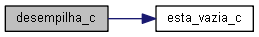
\includegraphics[width=266pt]{_pilha__c__func_8c_a53f4387852673f6e27870e3f05408aeb_cgraph}
\end{center}
\end{figure}
Here is the caller graph for this function\+:
\nopagebreak
\begin{figure}[H]
\begin{center}
\leavevmode
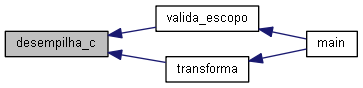
\includegraphics[width=344pt]{_pilha__c__func_8c_a53f4387852673f6e27870e3f05408aeb_icgraph}
\end{center}
\end{figure}
\mbox{\Hypertarget{_pilha__c__func_8c_a6b3dbcbb549fcd84a7e5aa1207dbc63c}\label{_pilha__c__func_8c_a6b3dbcbb549fcd84a7e5aa1207dbc63c}} 
\index{Pilha\+\_\+c\+\_\+func.\+c@{Pilha\+\_\+c\+\_\+func.\+c}!empilha\+\_\+c@{empilha\+\_\+c}}
\index{empilha\+\_\+c@{empilha\+\_\+c}!Pilha\+\_\+c\+\_\+func.\+c@{Pilha\+\_\+c\+\_\+func.\+c}}
\subsubsection{\texorpdfstring{empilha\+\_\+c()}{empilha\_c()}}
{\footnotesize\ttfamily int empilha\+\_\+c (\begin{DoxyParamCaption}\item[{char}]{dado,  }\item[{\mbox{\hyperlink{structt__pilha__c}{t\+\_\+pilha\+\_\+c}} $\ast$}]{pilha\+\_\+c }\end{DoxyParamCaption})}



Definition at line 37 of file Pilha\+\_\+c\+\_\+func.\+c.

Here is the call graph for this function\+:
\nopagebreak
\begin{figure}[H]
\begin{center}
\leavevmode
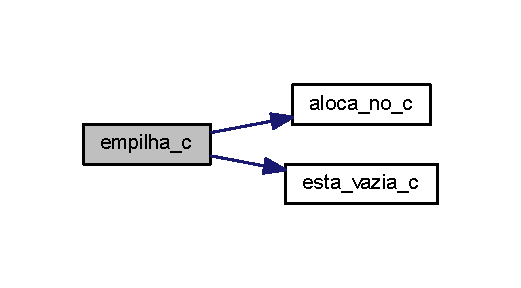
\includegraphics[width=250pt]{_pilha__c__func_8c_a6b3dbcbb549fcd84a7e5aa1207dbc63c_cgraph}
\end{center}
\end{figure}
Here is the caller graph for this function\+:
\nopagebreak
\begin{figure}[H]
\begin{center}
\leavevmode
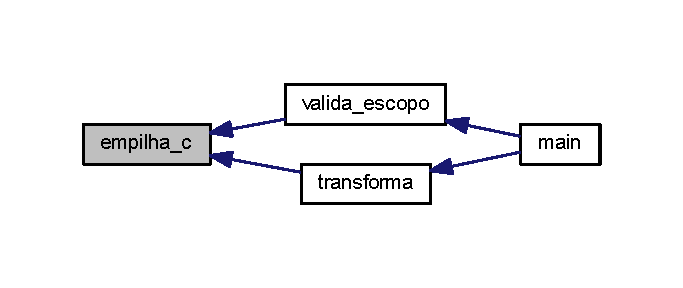
\includegraphics[width=328pt]{_pilha__c__func_8c_a6b3dbcbb549fcd84a7e5aa1207dbc63c_icgraph}
\end{center}
\end{figure}
\mbox{\Hypertarget{_pilha__c__func_8c_a28d30a9fcbf08a1f95ac47993a89acfc}\label{_pilha__c__func_8c_a28d30a9fcbf08a1f95ac47993a89acfc}} 
\index{Pilha\+\_\+c\+\_\+func.\+c@{Pilha\+\_\+c\+\_\+func.\+c}!esta\+\_\+vazia\+\_\+c@{esta\+\_\+vazia\+\_\+c}}
\index{esta\+\_\+vazia\+\_\+c@{esta\+\_\+vazia\+\_\+c}!Pilha\+\_\+c\+\_\+func.\+c@{Pilha\+\_\+c\+\_\+func.\+c}}
\subsubsection{\texorpdfstring{esta\+\_\+vazia\+\_\+c()}{esta\_vazia\_c()}}
{\footnotesize\ttfamily int esta\+\_\+vazia\+\_\+c (\begin{DoxyParamCaption}\item[{\mbox{\hyperlink{structt__pilha__c}{t\+\_\+pilha\+\_\+c}} $\ast$}]{pilha\+\_\+c }\end{DoxyParamCaption})}



Definition at line 102 of file Pilha\+\_\+c\+\_\+func.\+c.

Here is the caller graph for this function\+:
\nopagebreak
\begin{figure}[H]
\begin{center}
\leavevmode
\includegraphics[width=350pt]{_pilha__c__func_8c_a28d30a9fcbf08a1f95ac47993a89acfc_icgraph}
\end{center}
\end{figure}

\hypertarget{_pilha__func_8c}{}\section{Pilha\+\_\+func.\+c File Reference}
\label{_pilha__func_8c}\index{Pilha\+\_\+func.\+c@{Pilha\+\_\+func.\+c}}
{\ttfamily \#include \char`\"{}Calculadora.\+h\char`\"{}}\newline
Include dependency graph for Pilha\+\_\+func.\+c\+:
\nopagebreak
\begin{figure}[H]
\begin{center}
\leavevmode
\includegraphics[width=350pt]{_pilha__func_8c__incl}
\end{center}
\end{figure}
\subsection*{Functions}
\begin{DoxyCompactItemize}
\item 
\mbox{\hyperlink{structt__pilha}{t\+\_\+pilha}} $\ast$ \mbox{\hyperlink{_pilha__func_8c_a882b64f15d2cb66bbaeb41a341e71dce}{aloca\+\_\+pilha}} ()
\item 
\mbox{\hyperlink{_calculadora_8h_a312f04dbe081fc59526dcf1463e3380a}{t\+\_\+no}} $\ast$ \mbox{\hyperlink{_pilha__func_8c_ade7db9766f53662f025a944b636f4db2}{aloca\+\_\+no}} (float dado)
\item 
int \mbox{\hyperlink{_pilha__func_8c_a5705252b26adc92c6a848252ca1790c1}{empilha}} (float dado, \mbox{\hyperlink{structt__pilha}{t\+\_\+pilha}} $\ast$pilha)
\item 
void \mbox{\hyperlink{_pilha__func_8c_a7754e1e0150be8a3a784d637ed83a699}{imprime\+\_\+pilha}} (\mbox{\hyperlink{structt__pilha}{t\+\_\+pilha}} $\ast$pilha)
\item 
int \mbox{\hyperlink{_pilha__func_8c_adfd347e2b3f0462a4a1bd85e7d033e68}{esta\+\_\+vazia}} (\mbox{\hyperlink{structt__pilha}{t\+\_\+pilha}} $\ast$pilha)
\item 
void \mbox{\hyperlink{_pilha__func_8c_a5c485ba4895206b77485169e4d240157}{apaga\+\_\+pilha}} (\mbox{\hyperlink{structt__pilha}{t\+\_\+pilha}} $\ast$pilha)
\item 
int \mbox{\hyperlink{_pilha__func_8c_a91d1e173ad5aaecf8348f4429f54c210}{verifica\+\_\+pilha}} (\mbox{\hyperlink{structt__pilha}{t\+\_\+pilha}} $\ast$pilha)
\item 
float \mbox{\hyperlink{_pilha__func_8c_a0ce03f1f3ee5207eb5390b0658d1ca69}{desempilha\+\_\+e\+\_\+calcula\+\_\+1}} (char op, \mbox{\hyperlink{structt__pilha}{t\+\_\+pilha}} $\ast$pilha)
\item 
float \mbox{\hyperlink{_pilha__func_8c_a23bb611728759ee2acc8523f39b3b34c}{desempilha\+\_\+e\+\_\+calcula\+\_\+2}} (char op, \mbox{\hyperlink{structt__pilha}{t\+\_\+pilha}} $\ast$pilha)
\item 
int \mbox{\hyperlink{_pilha__func_8c_a9a11eff29728678483ea05fa1983018c}{remove\+\_\+ultimo}} (\mbox{\hyperlink{structt__pilha}{t\+\_\+pilha}} $\ast$pilha)
\end{DoxyCompactItemize}


\subsection{Function Documentation}
\mbox{\Hypertarget{_pilha__func_8c_ade7db9766f53662f025a944b636f4db2}\label{_pilha__func_8c_ade7db9766f53662f025a944b636f4db2}} 
\index{Pilha\+\_\+func.\+c@{Pilha\+\_\+func.\+c}!aloca\+\_\+no@{aloca\+\_\+no}}
\index{aloca\+\_\+no@{aloca\+\_\+no}!Pilha\+\_\+func.\+c@{Pilha\+\_\+func.\+c}}
\subsubsection{\texorpdfstring{aloca\+\_\+no()}{aloca\_no()}}
{\footnotesize\ttfamily \mbox{\hyperlink{_calculadora_8h_a312f04dbe081fc59526dcf1463e3380a}{t\+\_\+no}}$\ast$ aloca\+\_\+no (\begin{DoxyParamCaption}\item[{float}]{dado }\end{DoxyParamCaption})}



Definition at line 19 of file Pilha\+\_\+func.\+c.

Here is the caller graph for this function\+:
\nopagebreak
\begin{figure}[H]
\begin{center}
\leavevmode
\includegraphics[width=350pt]{_pilha__func_8c_ade7db9766f53662f025a944b636f4db2_icgraph}
\end{center}
\end{figure}
\mbox{\Hypertarget{_pilha__func_8c_a882b64f15d2cb66bbaeb41a341e71dce}\label{_pilha__func_8c_a882b64f15d2cb66bbaeb41a341e71dce}} 
\index{Pilha\+\_\+func.\+c@{Pilha\+\_\+func.\+c}!aloca\+\_\+pilha@{aloca\+\_\+pilha}}
\index{aloca\+\_\+pilha@{aloca\+\_\+pilha}!Pilha\+\_\+func.\+c@{Pilha\+\_\+func.\+c}}
\subsubsection{\texorpdfstring{aloca\+\_\+pilha()}{aloca\_pilha()}}
{\footnotesize\ttfamily \mbox{\hyperlink{structt__pilha}{t\+\_\+pilha}}$\ast$ aloca\+\_\+pilha (\begin{DoxyParamCaption}{ }\end{DoxyParamCaption})}



Definition at line 9 of file Pilha\+\_\+func.\+c.

Here is the caller graph for this function\+:
\nopagebreak
\begin{figure}[H]
\begin{center}
\leavevmode
\includegraphics[width=338pt]{_pilha__func_8c_a882b64f15d2cb66bbaeb41a341e71dce_icgraph}
\end{center}
\end{figure}
\mbox{\Hypertarget{_pilha__func_8c_a5c485ba4895206b77485169e4d240157}\label{_pilha__func_8c_a5c485ba4895206b77485169e4d240157}} 
\index{Pilha\+\_\+func.\+c@{Pilha\+\_\+func.\+c}!apaga\+\_\+pilha@{apaga\+\_\+pilha}}
\index{apaga\+\_\+pilha@{apaga\+\_\+pilha}!Pilha\+\_\+func.\+c@{Pilha\+\_\+func.\+c}}
\subsubsection{\texorpdfstring{apaga\+\_\+pilha()}{apaga\_pilha()}}
{\footnotesize\ttfamily void apaga\+\_\+pilha (\begin{DoxyParamCaption}\item[{\mbox{\hyperlink{structt__pilha}{t\+\_\+pilha}} $\ast$}]{pilha }\end{DoxyParamCaption})}



Definition at line 81 of file Pilha\+\_\+func.\+c.

Here is the caller graph for this function\+:
\nopagebreak
\begin{figure}[H]
\begin{center}
\leavevmode
\includegraphics[width=222pt]{_pilha__func_8c_a5c485ba4895206b77485169e4d240157_icgraph}
\end{center}
\end{figure}
\mbox{\Hypertarget{_pilha__func_8c_a0ce03f1f3ee5207eb5390b0658d1ca69}\label{_pilha__func_8c_a0ce03f1f3ee5207eb5390b0658d1ca69}} 
\index{Pilha\+\_\+func.\+c@{Pilha\+\_\+func.\+c}!desempilha\+\_\+e\+\_\+calcula\+\_\+1@{desempilha\+\_\+e\+\_\+calcula\+\_\+1}}
\index{desempilha\+\_\+e\+\_\+calcula\+\_\+1@{desempilha\+\_\+e\+\_\+calcula\+\_\+1}!Pilha\+\_\+func.\+c@{Pilha\+\_\+func.\+c}}
\subsubsection{\texorpdfstring{desempilha\+\_\+e\+\_\+calcula\+\_\+1()}{desempilha\_e\_calcula\_1()}}
{\footnotesize\ttfamily float desempilha\+\_\+e\+\_\+calcula\+\_\+1 (\begin{DoxyParamCaption}\item[{char}]{op,  }\item[{\mbox{\hyperlink{structt__pilha}{t\+\_\+pilha}} $\ast$}]{pilha }\end{DoxyParamCaption})}



Definition at line 107 of file Pilha\+\_\+func.\+c.

Here is the call graph for this function\+:
\nopagebreak
\begin{figure}[H]
\begin{center}
\leavevmode
\includegraphics[width=350pt]{_pilha__func_8c_a0ce03f1f3ee5207eb5390b0658d1ca69_cgraph}
\end{center}
\end{figure}
Here is the caller graph for this function\+:
\nopagebreak
\begin{figure}[H]
\begin{center}
\leavevmode
\includegraphics[width=350pt]{_pilha__func_8c_a0ce03f1f3ee5207eb5390b0658d1ca69_icgraph}
\end{center}
\end{figure}
\mbox{\Hypertarget{_pilha__func_8c_a23bb611728759ee2acc8523f39b3b34c}\label{_pilha__func_8c_a23bb611728759ee2acc8523f39b3b34c}} 
\index{Pilha\+\_\+func.\+c@{Pilha\+\_\+func.\+c}!desempilha\+\_\+e\+\_\+calcula\+\_\+2@{desempilha\+\_\+e\+\_\+calcula\+\_\+2}}
\index{desempilha\+\_\+e\+\_\+calcula\+\_\+2@{desempilha\+\_\+e\+\_\+calcula\+\_\+2}!Pilha\+\_\+func.\+c@{Pilha\+\_\+func.\+c}}
\subsubsection{\texorpdfstring{desempilha\+\_\+e\+\_\+calcula\+\_\+2()}{desempilha\_e\_calcula\_2()}}
{\footnotesize\ttfamily float desempilha\+\_\+e\+\_\+calcula\+\_\+2 (\begin{DoxyParamCaption}\item[{char}]{op,  }\item[{\mbox{\hyperlink{structt__pilha}{t\+\_\+pilha}} $\ast$}]{pilha }\end{DoxyParamCaption})}



Definition at line 164 of file Pilha\+\_\+func.\+c.

Here is the call graph for this function\+:
\nopagebreak
\begin{figure}[H]
\begin{center}
\leavevmode
\includegraphics[width=350pt]{_pilha__func_8c_a23bb611728759ee2acc8523f39b3b34c_cgraph}
\end{center}
\end{figure}
Here is the caller graph for this function\+:
\nopagebreak
\begin{figure}[H]
\begin{center}
\leavevmode
\includegraphics[width=277pt]{_pilha__func_8c_a23bb611728759ee2acc8523f39b3b34c_icgraph}
\end{center}
\end{figure}
\mbox{\Hypertarget{_pilha__func_8c_a5705252b26adc92c6a848252ca1790c1}\label{_pilha__func_8c_a5705252b26adc92c6a848252ca1790c1}} 
\index{Pilha\+\_\+func.\+c@{Pilha\+\_\+func.\+c}!empilha@{empilha}}
\index{empilha@{empilha}!Pilha\+\_\+func.\+c@{Pilha\+\_\+func.\+c}}
\subsubsection{\texorpdfstring{empilha()}{empilha()}}
{\footnotesize\ttfamily int empilha (\begin{DoxyParamCaption}\item[{float}]{dado,  }\item[{\mbox{\hyperlink{structt__pilha}{t\+\_\+pilha}} $\ast$}]{pilha }\end{DoxyParamCaption})}



Definition at line 34 of file Pilha\+\_\+func.\+c.

Here is the call graph for this function\+:
\nopagebreak
\begin{figure}[H]
\begin{center}
\leavevmode
\includegraphics[width=228pt]{_pilha__func_8c_a5705252b26adc92c6a848252ca1790c1_cgraph}
\end{center}
\end{figure}
Here is the caller graph for this function\+:
\nopagebreak
\begin{figure}[H]
\begin{center}
\leavevmode
\includegraphics[width=325pt]{_pilha__func_8c_a5705252b26adc92c6a848252ca1790c1_icgraph}
\end{center}
\end{figure}
\mbox{\Hypertarget{_pilha__func_8c_adfd347e2b3f0462a4a1bd85e7d033e68}\label{_pilha__func_8c_adfd347e2b3f0462a4a1bd85e7d033e68}} 
\index{Pilha\+\_\+func.\+c@{Pilha\+\_\+func.\+c}!esta\+\_\+vazia@{esta\+\_\+vazia}}
\index{esta\+\_\+vazia@{esta\+\_\+vazia}!Pilha\+\_\+func.\+c@{Pilha\+\_\+func.\+c}}
\subsubsection{\texorpdfstring{esta\+\_\+vazia()}{esta\_vazia()}}
{\footnotesize\ttfamily int esta\+\_\+vazia (\begin{DoxyParamCaption}\item[{\mbox{\hyperlink{structt__pilha}{t\+\_\+pilha}} $\ast$}]{pilha }\end{DoxyParamCaption})}



Definition at line 76 of file Pilha\+\_\+func.\+c.

Here is the caller graph for this function\+:
\nopagebreak
\begin{figure}[H]
\begin{center}
\leavevmode
\includegraphics[width=350pt]{_pilha__func_8c_adfd347e2b3f0462a4a1bd85e7d033e68_icgraph}
\end{center}
\end{figure}
\mbox{\Hypertarget{_pilha__func_8c_a7754e1e0150be8a3a784d637ed83a699}\label{_pilha__func_8c_a7754e1e0150be8a3a784d637ed83a699}} 
\index{Pilha\+\_\+func.\+c@{Pilha\+\_\+func.\+c}!imprime\+\_\+pilha@{imprime\+\_\+pilha}}
\index{imprime\+\_\+pilha@{imprime\+\_\+pilha}!Pilha\+\_\+func.\+c@{Pilha\+\_\+func.\+c}}
\subsubsection{\texorpdfstring{imprime\+\_\+pilha()}{imprime\_pilha()}}
{\footnotesize\ttfamily void imprime\+\_\+pilha (\begin{DoxyParamCaption}\item[{\mbox{\hyperlink{structt__pilha}{t\+\_\+pilha}} $\ast$}]{pilha }\end{DoxyParamCaption})}



Definition at line 60 of file Pilha\+\_\+func.\+c.

Here is the call graph for this function\+:
\nopagebreak
\begin{figure}[H]
\begin{center}
\leavevmode
\includegraphics[width=255pt]{_pilha__func_8c_a7754e1e0150be8a3a784d637ed83a699_cgraph}
\end{center}
\end{figure}
Here is the caller graph for this function\+:
\nopagebreak
\begin{figure}[H]
\begin{center}
\leavevmode
\includegraphics[width=231pt]{_pilha__func_8c_a7754e1e0150be8a3a784d637ed83a699_icgraph}
\end{center}
\end{figure}
\mbox{\Hypertarget{_pilha__func_8c_a9a11eff29728678483ea05fa1983018c}\label{_pilha__func_8c_a9a11eff29728678483ea05fa1983018c}} 
\index{Pilha\+\_\+func.\+c@{Pilha\+\_\+func.\+c}!remove\+\_\+ultimo@{remove\+\_\+ultimo}}
\index{remove\+\_\+ultimo@{remove\+\_\+ultimo}!Pilha\+\_\+func.\+c@{Pilha\+\_\+func.\+c}}
\subsubsection{\texorpdfstring{remove\+\_\+ultimo()}{remove\_ultimo()}}
{\footnotesize\ttfamily int remove\+\_\+ultimo (\begin{DoxyParamCaption}\item[{\mbox{\hyperlink{structt__pilha}{t\+\_\+pilha}} $\ast$}]{pilha }\end{DoxyParamCaption})}



Definition at line 221 of file Pilha\+\_\+func.\+c.

Here is the call graph for this function\+:
\nopagebreak
\begin{figure}[H]
\begin{center}
\leavevmode
\includegraphics[width=257pt]{_pilha__func_8c_a9a11eff29728678483ea05fa1983018c_cgraph}
\end{center}
\end{figure}
Here is the caller graph for this function\+:
\nopagebreak
\begin{figure}[H]
\begin{center}
\leavevmode
\includegraphics[width=350pt]{_pilha__func_8c_a9a11eff29728678483ea05fa1983018c_icgraph}
\end{center}
\end{figure}
\mbox{\Hypertarget{_pilha__func_8c_a91d1e173ad5aaecf8348f4429f54c210}\label{_pilha__func_8c_a91d1e173ad5aaecf8348f4429f54c210}} 
\index{Pilha\+\_\+func.\+c@{Pilha\+\_\+func.\+c}!verifica\+\_\+pilha@{verifica\+\_\+pilha}}
\index{verifica\+\_\+pilha@{verifica\+\_\+pilha}!Pilha\+\_\+func.\+c@{Pilha\+\_\+func.\+c}}
\subsubsection{\texorpdfstring{verifica\+\_\+pilha()}{verifica\_pilha()}}
{\footnotesize\ttfamily int verifica\+\_\+pilha (\begin{DoxyParamCaption}\item[{\mbox{\hyperlink{structt__pilha}{t\+\_\+pilha}} $\ast$}]{pilha }\end{DoxyParamCaption})}



Definition at line 97 of file Pilha\+\_\+func.\+c.

Here is the caller graph for this function\+:
\nopagebreak
\begin{figure}[H]
\begin{center}
\leavevmode
\includegraphics[width=344pt]{_pilha__func_8c_a91d1e173ad5aaecf8348f4429f54c210_icgraph}
\end{center}
\end{figure}

\hypertarget{_res__exp_8h}{}\section{Res\+\_\+exp.\+h File Reference}
\label{_res__exp_8h}\index{Res\+\_\+exp.\+h@{Res\+\_\+exp.\+h}}
{\ttfamily \#include $<$stdio.\+h$>$}\newline
{\ttfamily \#include $<$stdlib.\+h$>$}\newline
{\ttfamily \#include $<$string.\+h$>$}\newline
{\ttfamily \#include $<$stdbool.\+h$>$}\newline
{\ttfamily \#include $<$ctype.\+h$>$}\newline
Include dependency graph for Res\+\_\+exp.\+h\+:
\nopagebreak
\begin{figure}[H]
\begin{center}
\leavevmode
\includegraphics[width=350pt]{_res__exp_8h__incl}
\end{center}
\end{figure}
This graph shows which files directly or indirectly include this file\+:
\nopagebreak
\begin{figure}[H]
\begin{center}
\leavevmode
\includegraphics[width=350pt]{_res__exp_8h__dep__incl}
\end{center}
\end{figure}
\subsection*{Data Structures}
\begin{DoxyCompactItemize}
\item 
struct \mbox{\hyperlink{structno__c}{no\+\_\+c}}
\item 
struct \mbox{\hyperlink{structt__pilha__c}{t\+\_\+pilha\+\_\+c}}
\end{DoxyCompactItemize}
\subsection*{Typedefs}
\begin{DoxyCompactItemize}
\item 
typedef struct \mbox{\hyperlink{structno__c}{no\+\_\+c}} \mbox{\hyperlink{_res__exp_8h_a49875fde21799e17a8437b9caf0ec7d0}{t\+\_\+no\+\_\+c}}
\end{DoxyCompactItemize}
\subsection*{Functions}
\begin{DoxyCompactItemize}
\item 
\mbox{\hyperlink{structt__pilha__c}{t\+\_\+pilha\+\_\+c}} $\ast$ \mbox{\hyperlink{_res__exp_8h_ae39ed0ad591d07a0c9fde8b10b285b43}{aloca\+\_\+pilha\+\_\+c}} ()
\item 
\mbox{\hyperlink{_res__exp_8h_a49875fde21799e17a8437b9caf0ec7d0}{t\+\_\+no\+\_\+c}} $\ast$ \mbox{\hyperlink{_res__exp_8h_ae39c6a9b3cac787d0587ac6168ede0f4}{aloca\+\_\+no\+\_\+c}} (char dado)
\item 
int \mbox{\hyperlink{_res__exp_8h_a28d30a9fcbf08a1f95ac47993a89acfc}{esta\+\_\+vazia\+\_\+c}} (\mbox{\hyperlink{structt__pilha__c}{t\+\_\+pilha\+\_\+c}} $\ast$pilha\+\_\+c)
\item 
void \mbox{\hyperlink{_res__exp_8h_aeb21de9a00099b2715658d50ec54c6e5}{apaga\+\_\+pilha\+\_\+c}} (\mbox{\hyperlink{structt__pilha__c}{t\+\_\+pilha\+\_\+c}} $\ast$pilha\+\_\+c)
\item 
int \mbox{\hyperlink{_res__exp_8h_a6b3dbcbb549fcd84a7e5aa1207dbc63c}{empilha\+\_\+c}} (char dado, \mbox{\hyperlink{structt__pilha__c}{t\+\_\+pilha\+\_\+c}} $\ast$pilha\+\_\+c)
\item 
char \mbox{\hyperlink{_res__exp_8h_a53f4387852673f6e27870e3f05408aeb}{desempilha\+\_\+c}} (\mbox{\hyperlink{structt__pilha__c}{t\+\_\+pilha\+\_\+c}} $\ast$pilha\+\_\+c)
\item 
bool \mbox{\hyperlink{_res__exp_8h_abb9125d19fbf087fdf98a1d97c91d539}{valida\+\_\+str\+\_\+1}} (char c)
\item 
bool \mbox{\hyperlink{_res__exp_8h_ab8e6f6e06eb2f4abbaf7621baf85cd60}{tem\+\_\+numero}} (char c)
\item 
bool \mbox{\hyperlink{_res__exp_8h_a92c3c878a67583c49cb915e71346e832}{tem\+\_\+escopo}} (char c)
\item 
bool \mbox{\hyperlink{_res__exp_8h_a98aea14122474183a166bbd5ed65bca2}{tem\+\_\+op}} (char c)
\item 
int \mbox{\hyperlink{_res__exp_8h_a2c910b138da6936a83cb57fba3e3bdce}{check\+\_\+exp}} (char $\ast$str)
\item 
int \mbox{\hyperlink{_res__exp_8h_a0450cb0189bf507d2a9f8f057612d795}{valida\+\_\+escopo}} (char $\ast$str, \mbox{\hyperlink{structt__pilha__c}{t\+\_\+pilha\+\_\+c}} $\ast$pilha\+\_\+c)
\item 
int \mbox{\hyperlink{_res__exp_8h_ad0acd78bee8a5b768d35240be8cfb722}{precedencia}} (char c)
\item 
void \mbox{\hyperlink{_res__exp_8h_af2b0252508c5721283cdbdec77164236}{transforma}} (char $\ast$exp\+\_\+infixa, char $\ast$exp\+\_\+posfixa)
\item 
float \mbox{\hyperlink{_res__exp_8h_adb2dfa0d22377e798817bd431985a9e3}{resolve\+\_\+posfixa}} (char $\ast$str)
\end{DoxyCompactItemize}


\subsection{Typedef Documentation}
\mbox{\Hypertarget{_res__exp_8h_a49875fde21799e17a8437b9caf0ec7d0}\label{_res__exp_8h_a49875fde21799e17a8437b9caf0ec7d0}} 
\index{Res\+\_\+exp.\+h@{Res\+\_\+exp.\+h}!t\+\_\+no\+\_\+c@{t\+\_\+no\+\_\+c}}
\index{t\+\_\+no\+\_\+c@{t\+\_\+no\+\_\+c}!Res\+\_\+exp.\+h@{Res\+\_\+exp.\+h}}
\subsubsection{\texorpdfstring{t\+\_\+no\+\_\+c}{t\_no\_c}}
{\footnotesize\ttfamily typedef struct \mbox{\hyperlink{structno__c}{no\+\_\+c}} \mbox{\hyperlink{_res__exp_8h_a49875fde21799e17a8437b9caf0ec7d0}{t\+\_\+no\+\_\+c}}}



\subsection{Function Documentation}
\mbox{\Hypertarget{_res__exp_8h_ae39c6a9b3cac787d0587ac6168ede0f4}\label{_res__exp_8h_ae39c6a9b3cac787d0587ac6168ede0f4}} 
\index{Res\+\_\+exp.\+h@{Res\+\_\+exp.\+h}!aloca\+\_\+no\+\_\+c@{aloca\+\_\+no\+\_\+c}}
\index{aloca\+\_\+no\+\_\+c@{aloca\+\_\+no\+\_\+c}!Res\+\_\+exp.\+h@{Res\+\_\+exp.\+h}}
\subsubsection{\texorpdfstring{aloca\+\_\+no\+\_\+c()}{aloca\_no\_c()}}
{\footnotesize\ttfamily \mbox{\hyperlink{_res__exp_8h_a49875fde21799e17a8437b9caf0ec7d0}{t\+\_\+no\+\_\+c}}$\ast$ aloca\+\_\+no\+\_\+c (\begin{DoxyParamCaption}\item[{char}]{dado }\end{DoxyParamCaption})}



Definition at line 20 of file Pilha\+\_\+c\+\_\+func.\+c.

Here is the caller graph for this function\+:
\nopagebreak
\begin{figure}[H]
\begin{center}
\leavevmode
\includegraphics[width=350pt]{_res__exp_8h_ae39c6a9b3cac787d0587ac6168ede0f4_icgraph}
\end{center}
\end{figure}
\mbox{\Hypertarget{_res__exp_8h_ae39ed0ad591d07a0c9fde8b10b285b43}\label{_res__exp_8h_ae39ed0ad591d07a0c9fde8b10b285b43}} 
\index{Res\+\_\+exp.\+h@{Res\+\_\+exp.\+h}!aloca\+\_\+pilha\+\_\+c@{aloca\+\_\+pilha\+\_\+c}}
\index{aloca\+\_\+pilha\+\_\+c@{aloca\+\_\+pilha\+\_\+c}!Res\+\_\+exp.\+h@{Res\+\_\+exp.\+h}}
\subsubsection{\texorpdfstring{aloca\+\_\+pilha\+\_\+c()}{aloca\_pilha\_c()}}
{\footnotesize\ttfamily \mbox{\hyperlink{structt__pilha__c}{t\+\_\+pilha\+\_\+c}}$\ast$ aloca\+\_\+pilha\+\_\+c (\begin{DoxyParamCaption}{ }\end{DoxyParamCaption})}



Definition at line 9 of file Pilha\+\_\+c\+\_\+func.\+c.

Here is the caller graph for this function\+:
\nopagebreak
\begin{figure}[H]
\begin{center}
\leavevmode
\includegraphics[width=328pt]{_res__exp_8h_ae39ed0ad591d07a0c9fde8b10b285b43_icgraph}
\end{center}
\end{figure}
\mbox{\Hypertarget{_res__exp_8h_aeb21de9a00099b2715658d50ec54c6e5}\label{_res__exp_8h_aeb21de9a00099b2715658d50ec54c6e5}} 
\index{Res\+\_\+exp.\+h@{Res\+\_\+exp.\+h}!apaga\+\_\+pilha\+\_\+c@{apaga\+\_\+pilha\+\_\+c}}
\index{apaga\+\_\+pilha\+\_\+c@{apaga\+\_\+pilha\+\_\+c}!Res\+\_\+exp.\+h@{Res\+\_\+exp.\+h}}
\subsubsection{\texorpdfstring{apaga\+\_\+pilha\+\_\+c()}{apaga\_pilha\_c()}}
{\footnotesize\ttfamily void apaga\+\_\+pilha\+\_\+c (\begin{DoxyParamCaption}\item[{\mbox{\hyperlink{structt__pilha__c}{t\+\_\+pilha\+\_\+c}} $\ast$}]{pilha\+\_\+c }\end{DoxyParamCaption})}



Definition at line 107 of file Pilha\+\_\+c\+\_\+func.\+c.

Here is the caller graph for this function\+:
\nopagebreak
\begin{figure}[H]
\begin{center}
\leavevmode
\includegraphics[width=331pt]{_res__exp_8h_aeb21de9a00099b2715658d50ec54c6e5_icgraph}
\end{center}
\end{figure}
\mbox{\Hypertarget{_res__exp_8h_a2c910b138da6936a83cb57fba3e3bdce}\label{_res__exp_8h_a2c910b138da6936a83cb57fba3e3bdce}} 
\index{Res\+\_\+exp.\+h@{Res\+\_\+exp.\+h}!check\+\_\+exp@{check\+\_\+exp}}
\index{check\+\_\+exp@{check\+\_\+exp}!Res\+\_\+exp.\+h@{Res\+\_\+exp.\+h}}
\subsubsection{\texorpdfstring{check\+\_\+exp()}{check\_exp()}}
{\footnotesize\ttfamily int check\+\_\+exp (\begin{DoxyParamCaption}\item[{char $\ast$}]{str }\end{DoxyParamCaption})}



Definition at line 77 of file Valida\+\_\+exp\+\_\+func.\+c.

Here is the call graph for this function\+:
\nopagebreak
\begin{figure}[H]
\begin{center}
\leavevmode
\includegraphics[width=248pt]{_res__exp_8h_a2c910b138da6936a83cb57fba3e3bdce_cgraph}
\end{center}
\end{figure}
Here is the caller graph for this function\+:
\nopagebreak
\begin{figure}[H]
\begin{center}
\leavevmode
\includegraphics[width=218pt]{_res__exp_8h_a2c910b138da6936a83cb57fba3e3bdce_icgraph}
\end{center}
\end{figure}
\mbox{\Hypertarget{_res__exp_8h_a53f4387852673f6e27870e3f05408aeb}\label{_res__exp_8h_a53f4387852673f6e27870e3f05408aeb}} 
\index{Res\+\_\+exp.\+h@{Res\+\_\+exp.\+h}!desempilha\+\_\+c@{desempilha\+\_\+c}}
\index{desempilha\+\_\+c@{desempilha\+\_\+c}!Res\+\_\+exp.\+h@{Res\+\_\+exp.\+h}}
\subsubsection{\texorpdfstring{desempilha\+\_\+c()}{desempilha\_c()}}
{\footnotesize\ttfamily char desempilha\+\_\+c (\begin{DoxyParamCaption}\item[{\mbox{\hyperlink{structt__pilha__c}{t\+\_\+pilha\+\_\+c}} $\ast$}]{pilha\+\_\+c }\end{DoxyParamCaption})}



Definition at line 62 of file Pilha\+\_\+c\+\_\+func.\+c.

Here is the call graph for this function\+:
\nopagebreak
\begin{figure}[H]
\begin{center}
\leavevmode
\includegraphics[width=266pt]{_res__exp_8h_a53f4387852673f6e27870e3f05408aeb_cgraph}
\end{center}
\end{figure}
Here is the caller graph for this function\+:
\nopagebreak
\begin{figure}[H]
\begin{center}
\leavevmode
\includegraphics[width=344pt]{_res__exp_8h_a53f4387852673f6e27870e3f05408aeb_icgraph}
\end{center}
\end{figure}
\mbox{\Hypertarget{_res__exp_8h_a6b3dbcbb549fcd84a7e5aa1207dbc63c}\label{_res__exp_8h_a6b3dbcbb549fcd84a7e5aa1207dbc63c}} 
\index{Res\+\_\+exp.\+h@{Res\+\_\+exp.\+h}!empilha\+\_\+c@{empilha\+\_\+c}}
\index{empilha\+\_\+c@{empilha\+\_\+c}!Res\+\_\+exp.\+h@{Res\+\_\+exp.\+h}}
\subsubsection{\texorpdfstring{empilha\+\_\+c()}{empilha\_c()}}
{\footnotesize\ttfamily int empilha\+\_\+c (\begin{DoxyParamCaption}\item[{char}]{dado,  }\item[{\mbox{\hyperlink{structt__pilha__c}{t\+\_\+pilha\+\_\+c}} $\ast$}]{pilha\+\_\+c }\end{DoxyParamCaption})}



Definition at line 37 of file Pilha\+\_\+c\+\_\+func.\+c.

Here is the call graph for this function\+:
\nopagebreak
\begin{figure}[H]
\begin{center}
\leavevmode
\includegraphics[width=250pt]{_res__exp_8h_a6b3dbcbb549fcd84a7e5aa1207dbc63c_cgraph}
\end{center}
\end{figure}
Here is the caller graph for this function\+:
\nopagebreak
\begin{figure}[H]
\begin{center}
\leavevmode
\includegraphics[width=328pt]{_res__exp_8h_a6b3dbcbb549fcd84a7e5aa1207dbc63c_icgraph}
\end{center}
\end{figure}
\mbox{\Hypertarget{_res__exp_8h_a28d30a9fcbf08a1f95ac47993a89acfc}\label{_res__exp_8h_a28d30a9fcbf08a1f95ac47993a89acfc}} 
\index{Res\+\_\+exp.\+h@{Res\+\_\+exp.\+h}!esta\+\_\+vazia\+\_\+c@{esta\+\_\+vazia\+\_\+c}}
\index{esta\+\_\+vazia\+\_\+c@{esta\+\_\+vazia\+\_\+c}!Res\+\_\+exp.\+h@{Res\+\_\+exp.\+h}}
\subsubsection{\texorpdfstring{esta\+\_\+vazia\+\_\+c()}{esta\_vazia\_c()}}
{\footnotesize\ttfamily int esta\+\_\+vazia\+\_\+c (\begin{DoxyParamCaption}\item[{\mbox{\hyperlink{structt__pilha__c}{t\+\_\+pilha\+\_\+c}} $\ast$}]{pilha\+\_\+c }\end{DoxyParamCaption})}



Definition at line 102 of file Pilha\+\_\+c\+\_\+func.\+c.

Here is the caller graph for this function\+:
\nopagebreak
\begin{figure}[H]
\begin{center}
\leavevmode
\includegraphics[width=350pt]{_res__exp_8h_a28d30a9fcbf08a1f95ac47993a89acfc_icgraph}
\end{center}
\end{figure}
\mbox{\Hypertarget{_res__exp_8h_ad0acd78bee8a5b768d35240be8cfb722}\label{_res__exp_8h_ad0acd78bee8a5b768d35240be8cfb722}} 
\index{Res\+\_\+exp.\+h@{Res\+\_\+exp.\+h}!precedencia@{precedencia}}
\index{precedencia@{precedencia}!Res\+\_\+exp.\+h@{Res\+\_\+exp.\+h}}
\subsubsection{\texorpdfstring{precedencia()}{precedencia()}}
{\footnotesize\ttfamily int precedencia (\begin{DoxyParamCaption}\item[{char}]{c }\end{DoxyParamCaption})}



Definition at line 5 of file Algoritmo\+\_\+2.\+c.

Here is the caller graph for this function\+:
\nopagebreak
\begin{figure}[H]
\begin{center}
\leavevmode
\includegraphics[width=321pt]{_res__exp_8h_ad0acd78bee8a5b768d35240be8cfb722_icgraph}
\end{center}
\end{figure}
\mbox{\Hypertarget{_res__exp_8h_adb2dfa0d22377e798817bd431985a9e3}\label{_res__exp_8h_adb2dfa0d22377e798817bd431985a9e3}} 
\index{Res\+\_\+exp.\+h@{Res\+\_\+exp.\+h}!resolve\+\_\+posfixa@{resolve\+\_\+posfixa}}
\index{resolve\+\_\+posfixa@{resolve\+\_\+posfixa}!Res\+\_\+exp.\+h@{Res\+\_\+exp.\+h}}
\subsubsection{\texorpdfstring{resolve\+\_\+posfixa()}{resolve\_posfixa()}}
{\footnotesize\ttfamily float resolve\+\_\+posfixa (\begin{DoxyParamCaption}\item[{char $\ast$}]{str }\end{DoxyParamCaption})}



Definition at line 10 of file Algoritmo\+\_\+3.\+c.

Here is the call graph for this function\+:
\nopagebreak
\begin{figure}[H]
\begin{center}
\leavevmode
\includegraphics[width=350pt]{_res__exp_8h_adb2dfa0d22377e798817bd431985a9e3_cgraph}
\end{center}
\end{figure}
Here is the caller graph for this function\+:
\nopagebreak
\begin{figure}[H]
\begin{center}
\leavevmode
\includegraphics[width=237pt]{_res__exp_8h_adb2dfa0d22377e798817bd431985a9e3_icgraph}
\end{center}
\end{figure}
\mbox{\Hypertarget{_res__exp_8h_a92c3c878a67583c49cb915e71346e832}\label{_res__exp_8h_a92c3c878a67583c49cb915e71346e832}} 
\index{Res\+\_\+exp.\+h@{Res\+\_\+exp.\+h}!tem\+\_\+escopo@{tem\+\_\+escopo}}
\index{tem\+\_\+escopo@{tem\+\_\+escopo}!Res\+\_\+exp.\+h@{Res\+\_\+exp.\+h}}
\subsubsection{\texorpdfstring{tem\+\_\+escopo()}{tem\_escopo()}}
{\footnotesize\ttfamily bool tem\+\_\+escopo (\begin{DoxyParamCaption}\item[{char}]{c }\end{DoxyParamCaption})}



Definition at line 53 of file Valida\+\_\+exp\+\_\+func.\+c.

Here is the caller graph for this function\+:
\nopagebreak
\begin{figure}[H]
\begin{center}
\leavevmode
\includegraphics[width=337pt]{_res__exp_8h_a92c3c878a67583c49cb915e71346e832_icgraph}
\end{center}
\end{figure}
\mbox{\Hypertarget{_res__exp_8h_ab8e6f6e06eb2f4abbaf7621baf85cd60}\label{_res__exp_8h_ab8e6f6e06eb2f4abbaf7621baf85cd60}} 
\index{Res\+\_\+exp.\+h@{Res\+\_\+exp.\+h}!tem\+\_\+numero@{tem\+\_\+numero}}
\index{tem\+\_\+numero@{tem\+\_\+numero}!Res\+\_\+exp.\+h@{Res\+\_\+exp.\+h}}
\subsubsection{\texorpdfstring{tem\+\_\+numero()}{tem\_numero()}}
{\footnotesize\ttfamily bool tem\+\_\+numero (\begin{DoxyParamCaption}\item[{char}]{c }\end{DoxyParamCaption})}



Definition at line 35 of file Valida\+\_\+exp\+\_\+func.\+c.

Here is the caller graph for this function\+:
\nopagebreak
\begin{figure}[H]
\begin{center}
\leavevmode
\includegraphics[width=344pt]{_res__exp_8h_ab8e6f6e06eb2f4abbaf7621baf85cd60_icgraph}
\end{center}
\end{figure}
\mbox{\Hypertarget{_res__exp_8h_a98aea14122474183a166bbd5ed65bca2}\label{_res__exp_8h_a98aea14122474183a166bbd5ed65bca2}} 
\index{Res\+\_\+exp.\+h@{Res\+\_\+exp.\+h}!tem\+\_\+op@{tem\+\_\+op}}
\index{tem\+\_\+op@{tem\+\_\+op}!Res\+\_\+exp.\+h@{Res\+\_\+exp.\+h}}
\subsubsection{\texorpdfstring{tem\+\_\+op()}{tem\_op()}}
{\footnotesize\ttfamily bool tem\+\_\+op (\begin{DoxyParamCaption}\item[{char}]{c }\end{DoxyParamCaption})}



Definition at line 66 of file Valida\+\_\+exp\+\_\+func.\+c.

Here is the caller graph for this function\+:
\nopagebreak
\begin{figure}[H]
\begin{center}
\leavevmode
\includegraphics[width=322pt]{_res__exp_8h_a98aea14122474183a166bbd5ed65bca2_icgraph}
\end{center}
\end{figure}
\mbox{\Hypertarget{_res__exp_8h_af2b0252508c5721283cdbdec77164236}\label{_res__exp_8h_af2b0252508c5721283cdbdec77164236}} 
\index{Res\+\_\+exp.\+h@{Res\+\_\+exp.\+h}!transforma@{transforma}}
\index{transforma@{transforma}!Res\+\_\+exp.\+h@{Res\+\_\+exp.\+h}}
\subsubsection{\texorpdfstring{transforma()}{transforma()}}
{\footnotesize\ttfamily void transforma (\begin{DoxyParamCaption}\item[{char $\ast$}]{exp\+\_\+infixa,  }\item[{char $\ast$}]{exp\+\_\+posfixa }\end{DoxyParamCaption})}



Definition at line 18 of file Algoritmo\+\_\+2.\+c.

Here is the call graph for this function\+:
\nopagebreak
\begin{figure}[H]
\begin{center}
\leavevmode
\includegraphics[width=350pt]{_res__exp_8h_af2b0252508c5721283cdbdec77164236_cgraph}
\end{center}
\end{figure}
Here is the caller graph for this function\+:
\nopagebreak
\begin{figure}[H]
\begin{center}
\leavevmode
\includegraphics[width=216pt]{_res__exp_8h_af2b0252508c5721283cdbdec77164236_icgraph}
\end{center}
\end{figure}
\mbox{\Hypertarget{_res__exp_8h_a0450cb0189bf507d2a9f8f057612d795}\label{_res__exp_8h_a0450cb0189bf507d2a9f8f057612d795}} 
\index{Res\+\_\+exp.\+h@{Res\+\_\+exp.\+h}!valida\+\_\+escopo@{valida\+\_\+escopo}}
\index{valida\+\_\+escopo@{valida\+\_\+escopo}!Res\+\_\+exp.\+h@{Res\+\_\+exp.\+h}}
\subsubsection{\texorpdfstring{valida\+\_\+escopo()}{valida\_escopo()}}
{\footnotesize\ttfamily int valida\+\_\+escopo (\begin{DoxyParamCaption}\item[{char $\ast$}]{str,  }\item[{\mbox{\hyperlink{structt__pilha__c}{t\+\_\+pilha\+\_\+c}} $\ast$}]{pilha\+\_\+c }\end{DoxyParamCaption})}



Definition at line 6 of file Algoritmo\+\_\+1.\+c.

Here is the call graph for this function\+:
\nopagebreak
\begin{figure}[H]
\begin{center}
\leavevmode
\includegraphics[width=350pt]{_res__exp_8h_a0450cb0189bf507d2a9f8f057612d795_cgraph}
\end{center}
\end{figure}
Here is the caller graph for this function\+:
\nopagebreak
\begin{figure}[H]
\begin{center}
\leavevmode
\includegraphics[width=231pt]{_res__exp_8h_a0450cb0189bf507d2a9f8f057612d795_icgraph}
\end{center}
\end{figure}
\mbox{\Hypertarget{_res__exp_8h_abb9125d19fbf087fdf98a1d97c91d539}\label{_res__exp_8h_abb9125d19fbf087fdf98a1d97c91d539}} 
\index{Res\+\_\+exp.\+h@{Res\+\_\+exp.\+h}!valida\+\_\+str\+\_\+1@{valida\+\_\+str\+\_\+1}}
\index{valida\+\_\+str\+\_\+1@{valida\+\_\+str\+\_\+1}!Res\+\_\+exp.\+h@{Res\+\_\+exp.\+h}}
\subsubsection{\texorpdfstring{valida\+\_\+str\+\_\+1()}{valida\_str\_1()}}
{\footnotesize\ttfamily bool valida\+\_\+str\+\_\+1 (\begin{DoxyParamCaption}\item[{char}]{c }\end{DoxyParamCaption})}



Definition at line 7 of file Valida\+\_\+exp\+\_\+func.\+c.

Here is the caller graph for this function\+:
\nopagebreak
\begin{figure}[H]
\begin{center}
\leavevmode
\includegraphics[width=322pt]{_res__exp_8h_abb9125d19fbf087fdf98a1d97c91d539_icgraph}
\end{center}
\end{figure}

\hypertarget{_suporte__func_8c}{}\section{Suporte\+\_\+func.\+c File Reference}
\label{_suporte__func_8c}\index{Suporte\+\_\+func.\+c@{Suporte\+\_\+func.\+c}}
{\ttfamily \#include \char`\"{}Calculadora.\+h\char`\"{}}\newline
Include dependency graph for Suporte\+\_\+func.\+c\+:
\nopagebreak
\begin{figure}[H]
\begin{center}
\leavevmode
\includegraphics[width=350pt]{_suporte__func_8c__incl}
\end{center}
\end{figure}
\subsection*{Functions}
\begin{DoxyCompactItemize}
\item 
int \mbox{\hyperlink{_suporte__func_8c_a924e3344e312510ba6b0b0a1f63613d9}{copia\+\_\+elemento}} (\mbox{\hyperlink{structt__pilha}{t\+\_\+pilha}} $\ast$pilha)
\item 
void \mbox{\hyperlink{_suporte__func_8c_a7b541b1f54cc537f7b83b83b3b746a11}{limpabuffer}} ()
\item 
float \mbox{\hyperlink{_suporte__func_8c_aa670fb2fd144dab8265822c4e5f5f09c}{str\+\_\+em\+\_\+float}} (char $\ast$str)
\end{DoxyCompactItemize}


\subsection{Function Documentation}
\mbox{\Hypertarget{_suporte__func_8c_a924e3344e312510ba6b0b0a1f63613d9}\label{_suporte__func_8c_a924e3344e312510ba6b0b0a1f63613d9}} 
\index{Suporte\+\_\+func.\+c@{Suporte\+\_\+func.\+c}!copia\+\_\+elemento@{copia\+\_\+elemento}}
\index{copia\+\_\+elemento@{copia\+\_\+elemento}!Suporte\+\_\+func.\+c@{Suporte\+\_\+func.\+c}}
\subsubsection{\texorpdfstring{copia\+\_\+elemento()}{copia\_elemento()}}
{\footnotesize\ttfamily int copia\+\_\+elemento (\begin{DoxyParamCaption}\item[{\mbox{\hyperlink{structt__pilha}{t\+\_\+pilha}} $\ast$}]{pilha }\end{DoxyParamCaption})}



Definition at line 7 of file Suporte\+\_\+func.\+c.

Here is the call graph for this function\+:
\nopagebreak
\begin{figure}[H]
\begin{center}
\leavevmode
\includegraphics[width=350pt]{_suporte__func_8c_a924e3344e312510ba6b0b0a1f63613d9_cgraph}
\end{center}
\end{figure}
Here is the caller graph for this function\+:
\nopagebreak
\begin{figure}[H]
\begin{center}
\leavevmode
\includegraphics[width=239pt]{_suporte__func_8c_a924e3344e312510ba6b0b0a1f63613d9_icgraph}
\end{center}
\end{figure}
\mbox{\Hypertarget{_suporte__func_8c_a7b541b1f54cc537f7b83b83b3b746a11}\label{_suporte__func_8c_a7b541b1f54cc537f7b83b83b3b746a11}} 
\index{Suporte\+\_\+func.\+c@{Suporte\+\_\+func.\+c}!limpabuffer@{limpabuffer}}
\index{limpabuffer@{limpabuffer}!Suporte\+\_\+func.\+c@{Suporte\+\_\+func.\+c}}
\subsubsection{\texorpdfstring{limpabuffer()}{limpabuffer()}}
{\footnotesize\ttfamily void limpabuffer (\begin{DoxyParamCaption}{ }\end{DoxyParamCaption})}



Definition at line 33 of file Suporte\+\_\+func.\+c.

Here is the caller graph for this function\+:
\nopagebreak
\begin{figure}[H]
\begin{center}
\leavevmode
\includegraphics[width=217pt]{_suporte__func_8c_a7b541b1f54cc537f7b83b83b3b746a11_icgraph}
\end{center}
\end{figure}
\mbox{\Hypertarget{_suporte__func_8c_aa670fb2fd144dab8265822c4e5f5f09c}\label{_suporte__func_8c_aa670fb2fd144dab8265822c4e5f5f09c}} 
\index{Suporte\+\_\+func.\+c@{Suporte\+\_\+func.\+c}!str\+\_\+em\+\_\+float@{str\+\_\+em\+\_\+float}}
\index{str\+\_\+em\+\_\+float@{str\+\_\+em\+\_\+float}!Suporte\+\_\+func.\+c@{Suporte\+\_\+func.\+c}}
\subsubsection{\texorpdfstring{str\+\_\+em\+\_\+float()}{str\_em\_float()}}
{\footnotesize\ttfamily float str\+\_\+em\+\_\+float (\begin{DoxyParamCaption}\item[{char $\ast$}]{str }\end{DoxyParamCaption})}



Definition at line 39 of file Suporte\+\_\+func.\+c.

Here is the caller graph for this function\+:
\nopagebreak
\begin{figure}[H]
\begin{center}
\leavevmode
\includegraphics[width=343pt]{_suporte__func_8c_aa670fb2fd144dab8265822c4e5f5f09c_icgraph}
\end{center}
\end{figure}

\hypertarget{_valida__exp__func_8c}{}\section{Valida\+\_\+exp\+\_\+func.\+c File Reference}
\label{_valida__exp__func_8c}\index{Valida\+\_\+exp\+\_\+func.\+c@{Valida\+\_\+exp\+\_\+func.\+c}}
{\ttfamily \#include \char`\"{}Res\+\_\+exp.\+h\char`\"{}}\newline
Include dependency graph for Valida\+\_\+exp\+\_\+func.\+c\+:
\nopagebreak
\begin{figure}[H]
\begin{center}
\leavevmode
\includegraphics[width=350pt]{_valida__exp__func_8c__incl}
\end{center}
\end{figure}
\subsection*{Functions}
\begin{DoxyCompactItemize}
\item 
bool \mbox{\hyperlink{_valida__exp__func_8c_abb9125d19fbf087fdf98a1d97c91d539}{valida\+\_\+str\+\_\+1}} (char c)
\item 
bool \mbox{\hyperlink{_valida__exp__func_8c_ab8e6f6e06eb2f4abbaf7621baf85cd60}{tem\+\_\+numero}} (char c)
\item 
bool \mbox{\hyperlink{_valida__exp__func_8c_a92c3c878a67583c49cb915e71346e832}{tem\+\_\+escopo}} (char c)
\item 
bool \mbox{\hyperlink{_valida__exp__func_8c_a98aea14122474183a166bbd5ed65bca2}{tem\+\_\+op}} (char c)
\item 
int \mbox{\hyperlink{_valida__exp__func_8c_a2c910b138da6936a83cb57fba3e3bdce}{check\+\_\+exp}} (char $\ast$str)
\end{DoxyCompactItemize}


\subsection{Function Documentation}
\mbox{\Hypertarget{_valida__exp__func_8c_a2c910b138da6936a83cb57fba3e3bdce}\label{_valida__exp__func_8c_a2c910b138da6936a83cb57fba3e3bdce}} 
\index{Valida\+\_\+exp\+\_\+func.\+c@{Valida\+\_\+exp\+\_\+func.\+c}!check\+\_\+exp@{check\+\_\+exp}}
\index{check\+\_\+exp@{check\+\_\+exp}!Valida\+\_\+exp\+\_\+func.\+c@{Valida\+\_\+exp\+\_\+func.\+c}}
\subsubsection{\texorpdfstring{check\+\_\+exp()}{check\_exp()}}
{\footnotesize\ttfamily int check\+\_\+exp (\begin{DoxyParamCaption}\item[{char $\ast$}]{str }\end{DoxyParamCaption})}



Definition at line 77 of file Valida\+\_\+exp\+\_\+func.\+c.

Here is the call graph for this function\+:
\nopagebreak
\begin{figure}[H]
\begin{center}
\leavevmode
\includegraphics[width=248pt]{_valida__exp__func_8c_a2c910b138da6936a83cb57fba3e3bdce_cgraph}
\end{center}
\end{figure}
Here is the caller graph for this function\+:
\nopagebreak
\begin{figure}[H]
\begin{center}
\leavevmode
\includegraphics[width=218pt]{_valida__exp__func_8c_a2c910b138da6936a83cb57fba3e3bdce_icgraph}
\end{center}
\end{figure}
\mbox{\Hypertarget{_valida__exp__func_8c_a92c3c878a67583c49cb915e71346e832}\label{_valida__exp__func_8c_a92c3c878a67583c49cb915e71346e832}} 
\index{Valida\+\_\+exp\+\_\+func.\+c@{Valida\+\_\+exp\+\_\+func.\+c}!tem\+\_\+escopo@{tem\+\_\+escopo}}
\index{tem\+\_\+escopo@{tem\+\_\+escopo}!Valida\+\_\+exp\+\_\+func.\+c@{Valida\+\_\+exp\+\_\+func.\+c}}
\subsubsection{\texorpdfstring{tem\+\_\+escopo()}{tem\_escopo()}}
{\footnotesize\ttfamily bool tem\+\_\+escopo (\begin{DoxyParamCaption}\item[{char}]{c }\end{DoxyParamCaption})}



Definition at line 53 of file Valida\+\_\+exp\+\_\+func.\+c.

Here is the caller graph for this function\+:
\nopagebreak
\begin{figure}[H]
\begin{center}
\leavevmode
\includegraphics[width=337pt]{_valida__exp__func_8c_a92c3c878a67583c49cb915e71346e832_icgraph}
\end{center}
\end{figure}
\mbox{\Hypertarget{_valida__exp__func_8c_ab8e6f6e06eb2f4abbaf7621baf85cd60}\label{_valida__exp__func_8c_ab8e6f6e06eb2f4abbaf7621baf85cd60}} 
\index{Valida\+\_\+exp\+\_\+func.\+c@{Valida\+\_\+exp\+\_\+func.\+c}!tem\+\_\+numero@{tem\+\_\+numero}}
\index{tem\+\_\+numero@{tem\+\_\+numero}!Valida\+\_\+exp\+\_\+func.\+c@{Valida\+\_\+exp\+\_\+func.\+c}}
\subsubsection{\texorpdfstring{tem\+\_\+numero()}{tem\_numero()}}
{\footnotesize\ttfamily bool tem\+\_\+numero (\begin{DoxyParamCaption}\item[{char}]{c }\end{DoxyParamCaption})}



Definition at line 35 of file Valida\+\_\+exp\+\_\+func.\+c.

Here is the caller graph for this function\+:
\nopagebreak
\begin{figure}[H]
\begin{center}
\leavevmode
\includegraphics[width=344pt]{_valida__exp__func_8c_ab8e6f6e06eb2f4abbaf7621baf85cd60_icgraph}
\end{center}
\end{figure}
\mbox{\Hypertarget{_valida__exp__func_8c_a98aea14122474183a166bbd5ed65bca2}\label{_valida__exp__func_8c_a98aea14122474183a166bbd5ed65bca2}} 
\index{Valida\+\_\+exp\+\_\+func.\+c@{Valida\+\_\+exp\+\_\+func.\+c}!tem\+\_\+op@{tem\+\_\+op}}
\index{tem\+\_\+op@{tem\+\_\+op}!Valida\+\_\+exp\+\_\+func.\+c@{Valida\+\_\+exp\+\_\+func.\+c}}
\subsubsection{\texorpdfstring{tem\+\_\+op()}{tem\_op()}}
{\footnotesize\ttfamily bool tem\+\_\+op (\begin{DoxyParamCaption}\item[{char}]{c }\end{DoxyParamCaption})}



Definition at line 66 of file Valida\+\_\+exp\+\_\+func.\+c.

Here is the caller graph for this function\+:
\nopagebreak
\begin{figure}[H]
\begin{center}
\leavevmode
\includegraphics[width=322pt]{_valida__exp__func_8c_a98aea14122474183a166bbd5ed65bca2_icgraph}
\end{center}
\end{figure}
\mbox{\Hypertarget{_valida__exp__func_8c_abb9125d19fbf087fdf98a1d97c91d539}\label{_valida__exp__func_8c_abb9125d19fbf087fdf98a1d97c91d539}} 
\index{Valida\+\_\+exp\+\_\+func.\+c@{Valida\+\_\+exp\+\_\+func.\+c}!valida\+\_\+str\+\_\+1@{valida\+\_\+str\+\_\+1}}
\index{valida\+\_\+str\+\_\+1@{valida\+\_\+str\+\_\+1}!Valida\+\_\+exp\+\_\+func.\+c@{Valida\+\_\+exp\+\_\+func.\+c}}
\subsubsection{\texorpdfstring{valida\+\_\+str\+\_\+1()}{valida\_str\_1()}}
{\footnotesize\ttfamily bool valida\+\_\+str\+\_\+1 (\begin{DoxyParamCaption}\item[{char}]{c }\end{DoxyParamCaption})}



Definition at line 7 of file Valida\+\_\+exp\+\_\+func.\+c.

Here is the caller graph for this function\+:
\nopagebreak
\begin{figure}[H]
\begin{center}
\leavevmode
\includegraphics[width=322pt]{_valida__exp__func_8c_abb9125d19fbf087fdf98a1d97c91d539_icgraph}
\end{center}
\end{figure}

\hypertarget{_valida__func_8c}{}\section{Valida\+\_\+func.\+c File Reference}
\label{_valida__func_8c}\index{Valida\+\_\+func.\+c@{Valida\+\_\+func.\+c}}
{\ttfamily \#include \char`\"{}Calculadora.\+h\char`\"{}}\newline
Include dependency graph for Valida\+\_\+func.\+c\+:
\nopagebreak
\begin{figure}[H]
\begin{center}
\leavevmode
\includegraphics[width=350pt]{_valida__func_8c__incl}
\end{center}
\end{figure}
\subsection*{Functions}
\begin{DoxyCompactItemize}
\item 
bool \mbox{\hyperlink{_valida__func_8c_ac9a342197c376e2cd018f95b1394618c}{valida\+\_\+str}} (char c)
\item 
bool \mbox{\hyperlink{_valida__func_8c_a938fdba0cc830b48c5d0a85ad31c4bed}{tem\+\_\+char}} (char c)
\item 
bool \mbox{\hyperlink{_valida__func_8c_a6bdb02d6cf0aabad0986f4ed8f5a7056}{tem\+\_\+operador}} (char c)
\item 
int \mbox{\hyperlink{_valida__func_8c_a57b564d2fcef3dd2d88aa2fe653a7771}{check}} (char $\ast$str)
\end{DoxyCompactItemize}


\subsection{Function Documentation}
\mbox{\Hypertarget{_valida__func_8c_a57b564d2fcef3dd2d88aa2fe653a7771}\label{_valida__func_8c_a57b564d2fcef3dd2d88aa2fe653a7771}} 
\index{Valida\+\_\+func.\+c@{Valida\+\_\+func.\+c}!check@{check}}
\index{check@{check}!Valida\+\_\+func.\+c@{Valida\+\_\+func.\+c}}
\subsubsection{\texorpdfstring{check()}{check()}}
{\footnotesize\ttfamily int check (\begin{DoxyParamCaption}\item[{char $\ast$}]{str }\end{DoxyParamCaption})}



Definition at line 59 of file Valida\+\_\+func.\+c.

Here is the call graph for this function\+:
\nopagebreak
\begin{figure}[H]
\begin{center}
\leavevmode
\includegraphics[width=235pt]{_valida__func_8c_a57b564d2fcef3dd2d88aa2fe653a7771_cgraph}
\end{center}
\end{figure}
Here is the caller graph for this function\+:
\nopagebreak
\begin{figure}[H]
\begin{center}
\leavevmode
\includegraphics[width=197pt]{_valida__func_8c_a57b564d2fcef3dd2d88aa2fe653a7771_icgraph}
\end{center}
\end{figure}
\mbox{\Hypertarget{_valida__func_8c_a938fdba0cc830b48c5d0a85ad31c4bed}\label{_valida__func_8c_a938fdba0cc830b48c5d0a85ad31c4bed}} 
\index{Valida\+\_\+func.\+c@{Valida\+\_\+func.\+c}!tem\+\_\+char@{tem\+\_\+char}}
\index{tem\+\_\+char@{tem\+\_\+char}!Valida\+\_\+func.\+c@{Valida\+\_\+func.\+c}}
\subsubsection{\texorpdfstring{tem\+\_\+char()}{tem\_char()}}
{\footnotesize\ttfamily bool tem\+\_\+char (\begin{DoxyParamCaption}\item[{char}]{c }\end{DoxyParamCaption})}



Definition at line 32 of file Valida\+\_\+func.\+c.

Here is the caller graph for this function\+:
\nopagebreak
\begin{figure}[H]
\begin{center}
\leavevmode
\includegraphics[width=290pt]{_valida__func_8c_a938fdba0cc830b48c5d0a85ad31c4bed_icgraph}
\end{center}
\end{figure}
\mbox{\Hypertarget{_valida__func_8c_a6bdb02d6cf0aabad0986f4ed8f5a7056}\label{_valida__func_8c_a6bdb02d6cf0aabad0986f4ed8f5a7056}} 
\index{Valida\+\_\+func.\+c@{Valida\+\_\+func.\+c}!tem\+\_\+operador@{tem\+\_\+operador}}
\index{tem\+\_\+operador@{tem\+\_\+operador}!Valida\+\_\+func.\+c@{Valida\+\_\+func.\+c}}
\subsubsection{\texorpdfstring{tem\+\_\+operador()}{tem\_operador()}}
{\footnotesize\ttfamily bool tem\+\_\+operador (\begin{DoxyParamCaption}\item[{char}]{c }\end{DoxyParamCaption})}



Definition at line 46 of file Valida\+\_\+func.\+c.

Here is the caller graph for this function\+:
\nopagebreak
\begin{figure}[H]
\begin{center}
\leavevmode
\includegraphics[width=309pt]{_valida__func_8c_a6bdb02d6cf0aabad0986f4ed8f5a7056_icgraph}
\end{center}
\end{figure}
\mbox{\Hypertarget{_valida__func_8c_ac9a342197c376e2cd018f95b1394618c}\label{_valida__func_8c_ac9a342197c376e2cd018f95b1394618c}} 
\index{Valida\+\_\+func.\+c@{Valida\+\_\+func.\+c}!valida\+\_\+str@{valida\+\_\+str}}
\index{valida\+\_\+str@{valida\+\_\+str}!Valida\+\_\+func.\+c@{Valida\+\_\+func.\+c}}
\subsubsection{\texorpdfstring{valida\+\_\+str()}{valida\_str()}}
{\footnotesize\ttfamily bool valida\+\_\+str (\begin{DoxyParamCaption}\item[{char}]{c }\end{DoxyParamCaption})}



Definition at line 7 of file Valida\+\_\+func.\+c.

Here is the caller graph for this function\+:
\nopagebreak
\begin{figure}[H]
\begin{center}
\leavevmode
\includegraphics[width=290pt]{_valida__func_8c_ac9a342197c376e2cd018f95b1394618c_icgraph}
\end{center}
\end{figure}

%--- End generated contents ---

% Index
\backmatter
\newpage
\phantomsection
\clearemptydoublepage
\addcontentsline{toc}{chapter}{Index}
\printindex

\end{document}
